%%% Hlavní soubor. Zde se definují základní parametry a odkazuje se na ostatní části. %%%

%% Verze pro jednostranný tisk:
% Okraje: levý 40mm, pravý 25mm, horní a dolní 25mm
% (ale pozor, LaTeX si sám přidává 1in)
\documentclass[12pt,a4paper]{report}
\setlength\textwidth{145mm}
\setlength\textheight{247mm}
\setlength\oddsidemargin{15mm}
\setlength\evensidemargin{15mm}
\setlength\topmargin{0mm}
\setlength\headsep{0mm}
\setlength\headheight{0mm}
% \openright zařídí, aby následující text začínal na pravé straně knihy
\let\openright=\clearpage

\makeatletter
\newcommand\iraggedright{%
  \let\\\@centercr\@rightskip\@flushglue \rightskip\@rightskip
  \leftskip\z@skip}
\makeatother

%% Pokud tiskneme oboustranně:
% \documentclass[12pt,a4paper,twoside,openright]{report}
% \setlength\textwidth{145mm}
% \setlength\textheight{247mm}
% \setlength\oddsidemargin{14.2mm}
% \setlength\evensidemargin{0mm}
% \setlength\topmargin{0mm}
% \setlength\headsep{0mm}
% \setlength\headheight{0mm}
% \let\openright=\cleardoublepage

%% Vytváříme PDF/A-2u
\usepackage[a-2u]{pdfx}

%% Přepneme na českou sazbu a fonty Latin Modern
\usepackage[czech]{babel}
\usepackage{lmodern}
\usepackage[T1]{fontenc}
\usepackage{textcomp}

%% Použité kódování znaků: obvykle latin2, cp1250 nebo utf8:
\usepackage[utf8]{inputenc}

%%% Další užitečné balíčky (jsou součástí běžných distribucí LaTeXu)
\usepackage{amsmath}        % rozšíření pro sazbu matematiky
\usepackage{amsfonts}       % matematické fonty
\usepackage{amsthm}         % sazba vět, definic apod.
\usepackage{bbding}         % balíček s nejrůznějšími symboly
			    % (čtverečky, hvězdičky, tužtičky, nůžtičky, ...)
\usepackage{bm}             % tučné symboly (příkaz \bm)
\usepackage{graphicx}       % vkládání obrázků
\usepackage{fancyvrb}       % vylepšené prostředí pro strojové písmo
\usepackage{indentfirst}    % zavede odsazení 1. odstavce kapitoly

\usepackage[backend=biber]{biblatex}
%\usepackage{natbib}         % zajištuje možnost odkazovat na literaturu
			    % stylem AUTOR (ROK), resp. AUTOR [ČÍSLO]
\usepackage[nottoc]{tocbibind} % zajistí přidání seznamu literatury,
                            % obrázků a tabulek do obsahu
\usepackage{icomma}         % inteligetní čárka v matematickém módu
\usepackage{dcolumn}        % lepší zarovnání sloupců v tabulkách
\usepackage{booktabs}       % lepší vodorovné linky v tabulkách
\usepackage{paralist}       % lepší enumerate a itemize
\usepackage{xcolor}         % barevná sazba

\usepackage{hyperref}
\usepackage[none]{hyphenat}
\iraggedright
\usepackage{acro}	% seznam zkratek
\DeclareAcronym{FPS}{
    short=FPS,
    long=First Person Shooter - střílečka z pohledu první osoby,
}

\DeclareAcronym{RPG}{
    short=RPG,
    long=Role Playing Game - hra na hrdiny,
}
\DeclareAcronym{VR}{
    short=VR,
    long=Virtuální Realita,
}
\DeclareAcronym{LARP}{
    short=LARP,
    long=Live Action Role Playing,
}

\addbibresource{literatura.bib}
%%% Údaje o práci

% Název práce v jazyce práce (přesně podle zadání)
\def\NazevPrace{3D Simulátor šermu s mečem založený na fyzice}

% Název práce v angličtině
\def\NazevPraceEN{3D Physics driven swordfighting simulator}

% Jméno autora
\def\AutorPrace{Jakub Hroník}

% Rok odevzdání
\def\RokOdevzdani{2023}

% Název katedry nebo ústavu, kde byla práce oficiálně zadána
% (dle Organizační struktury MFF UK, případně plný název pracoviště mimo MFF)
\def\Katedra{Katedra softwaru a výuky informatiky}
\def\KatedraEN{Department of Software and Computer Science Education}

% Jedná se o katedru (department) nebo o ústav (institute)?
\def\TypPracoviste{Katedra}
\def\TypPracovisteEN{Department}

% Vedoucí práce: Jméno a příjmení s~tituly
\def\Vedouci{Mgr. Vojtěch Černý}

% Pracoviště vedoucího (opět dle Organizační struktury MFF)
\def\KatedraVedouciho{Katedra softwaru a výuky informatiky}
\def\KatedraVedoucihoEN{Department of Software and Computer Science Education}

% Studijní program a obor
\def\StudijniProgram{Informatika (B1801)}
\def\StudijniObor{IPSS (1801R048)}

% Nepovinné poděkování (vedoucímu práce, konzultantovi, tomu, kdo
% zapůjčil software, literaturu apod.)
\def\Podekovani{%
Poděkování.
}

% Abstrakt (doporučený rozsah cca 80-200 slov; nejedná se o zadání práce)
\def\Abstrakt{%
Boj nablízko s chladnou zbraní najdeme v mnoha videohrách, pouze hrstka z nich se však pokouší o realistickou simulaci, jež by hráči dala svobodu jakkoliv se blížící té, již manipulace s chladnou zbraní umožňuje v reálném světě. Velkou výzvou je návrh schématu ovládání pro klasické počítačové periferie. Ještě méně prozkoumanou oblastí je pak zapojení zbraně do fyzikální simulace herního světa.

Práce implementuje simulátor šermu s jedenapůlručním mečem v enginu Unity, v němž figuruje meč jako plně fyzikálně simulovaný objekt. Rovněž předkládá schéma ovládání pro klávesnici a myš umožňující hráči jemnou kontrolu nad pohybem zbraně. Pro testování hratelnosti implementuje jednoduchého AI protivníka.
Implementace je vytvořena s použitím dobrých programátorských praktik a může komukoliv posloužit jako základ pro akční hru s pokročilým bojovým systémem.
}
\def\AbstraktEN{%
--PLACEHOLDER--
}

% 3 až 5 klíčových slov (doporučeno), každé uzavřeno ve složených závorkách
\def\KlicovaSlova{%
{šerm} {herní fyzika} {počítačová hra} {herní engine Unity}
}
\def\KlicovaSlovaEN{%
{swordfighting} {game physics} {computer game} {Unity engine}
}

%% Balíček hyperref, kterým jdou vyrábět klikací odkazy v PDF,
%% ale hlavně ho používáme k uložení metadat do PDF (včetně obsahu).
%% Většinu nastavítek přednastaví balíček pdfx.
\hypersetup{unicode}
\hypersetup{breaklinks=true}

%% Definice různých užitečných maker (viz popis uvnitř souboru)
\include{makra}

%% Titulní strana a různé povinné informační strany
\begin{document}
\include{titulka}

%%% Strana s automaticky generovaným obsahem bakalářské práce

\tableofcontents

%%% Jednotlivé kapitoly práce jsou pro přehlednost uloženy v samostatných souborech
\chapter*{Úvod}
\addcontentsline{toc}{chapter}{Úvod}

Boj nablízko s chladnou zbraní je jev, kterým se zabývá mnoho videoher. Mezi žánry, které se na něj zaměřují, patří akční adventury, RPG a hack-n-slash. Důležitý koncept to je i pro žánr válečných strategických her, doplňující roli pak mívá například v FPS nebo stealth hrách. Zkrátka, pokud hra ztvárňuje nějaký konflikt řešený násilnou cestou, s vysokou pravděpodobností v ní nějaká chladná zbraň figuruje.

Herní mechaniky, skrz které je boj zblízka realizován, si od počátku éry videoher prošly složitou evolucí a samozřejmě každý žánr si je pojímá dost po svém aby ladily s jeho dalšími specifiky. I tak je ale překvapivě jednoduché popsat určité vlastnosti, které vykrystalizovaly jako společné jádro, které většinová část her sdílí.

Zpravidla zbraň ve hře funguje jako "černá skříňka" - hráč ji aktivuje stisknutím tlačítka - a postava zaútočí jak sama uzná za vhodné, například přehráním jedné ze seznamu předem připravených animací. Toto simplistické rozhraní má za výhody přívětivost a snadnou uchopitelnost pro nové hráče a také to, že na něj jde napasovat víceméně libovolná zbraň, od jednoručního meče přes halapartnu až po rozbitou sklenici od pálenky. Nevýhoda je pak ale, že vzniká výrazný rozdíl mezi tím, jak hráč hraje, a co postava dělá. Hráč tím pádem může cítit pocit nedostatečné kontroly a může trpět jeho imerze. Komerčně úspěšných her, které se pokusily hráči dát nad zbraní přímější kontrolu, najdeme v historii pouze několik [], celkově jde o oblast překvapivě málo prozkoumanou. 

Mezi očividné výzvy patří návrh schéma ovládání.  Klasicky používané periferie jako je počítačová myš či ovladač u herní konzole poskytují dvourozměrnou informaci, chladná zbraň je však obecný objekt v 3D prostoru s třemi úhly volnosti pro pohyb a dalšími třemi pro rotaci, z nichž žádný nemůžeme bez následků zanedbat. Je tedy zřejmé, že pomocí klasických periferií není možné dosáhnout dokonale jemného ovládání, které by bylo zároveň pro hráče intuitivní - je třeba nalézt vhodný kompromis. Alternativní periferie, které tento problém nemají, existují (zejména v oblasti Virtuální Reality), avšak stále nejsou natolik rozšířené, aby s nimi mohl počítat herní mainstream. Rovněž přinášejí své vlastní problémy. V dosavadních pokusech herních studií můžeme vidět velmi rozdílné způsoby jak k této výzvě přistupovaly. Každý exceluje v jiných situacích a má jiné očividné nedostatky, z pohledu na ně je zřejmé že tato oblast si vyžaduje další výzkum. 


\chapter{Základy}
V této kapitole uvedeme čtenáře do problematiky boje s chladnou zbraní - velmi stručně nastíníme jeho vývoj a metodiku v reálném světě a následně do hloubky rozebereme mechaniky, skrze které ho adaptuje svět akčních videoher, a problémy, které při tom musí řešit.


\section{Chladná zbraň v reálném světě}
V této sekci čtenáře velmi stručně seznámíme s historickým pozadím a základními charakteristikami, které provázejí boj s chladnou zbraní v reálném světě.

\subsection{Průlet historií}

Není nadsázkou když prohlásíme, že chladná zbraň je koncept starý jako lidstvo samo. Archelogické nálezy nasvědčují, že již vzdálený předek moderního člověka Australopithecus používal úderný předmět (pravděpodobně kus dřeva či kost ulovené antilopy) jako \textbf{nástroj k lovu} paviánů \cite{AustralopithecusWeapon}. \textbf{Výhody}, které mu to mohlo přinést, jsou zjevné: zatímco kořist měla možnosti obrany omezené tím, kam dosáhly její vlastní zuby a drápy, lovec si ji mohl držet v bezpečné vzdálenosti a vystavovat vlastní tělo o poznání menšímu nebezpečí odvety.

V průběhu svého vývoje lidský rod zdokonaloval i své zbraně, což přineslo mnoho dalších implikací - ostrý kamenný hrot člověku umožnil zasazovat ránu spolehlivě, a hlubší, než by kdy umožnilo pouhé jeho tělo. Spolehlivost zbraně umožnila lepší \textbf{koordinaci mezi lovci}. Sofistikovaná koordinace člověku otevřela cestu k lovu větších a silnějších druhů zvěře. Nakonec se člověk propracoval na samý vrchol potravního řetězce a zbraň, nástroj lovu, sloužila stále více pro vzájemný \textbf{boj mezi lidmi}. 

Zrod civilizací vznesl na zbraň nové požadavky. Vysoká koncentrace lidí na jednom místě vedla přirozeně ke specializaci profesí, mezi jinými i vojenské. \textbf{Profesionální armáda} čítající tisíce lidí umožňovala (a vyžadovala) do té doby nevídanou míru koordinace - ideálem v takové situaci se ukázalo disponovat širokou škálou zbraní vysoce specializovaných, chladných i střelných, jež mohly být použity ve vzájemné synergii, doplněné válečnými stroji a vhodně vycvičenými zvířaty\footnote{kůň jak známo hrál přední roli}. Profesionální voják měl čas a motivaci svůj typ zbraně pochopit do hloubky, stejně tak vysoce náročná si mohla dovolit být i její výroba a údržba, za níž nesli zodpovědnost rovněž profesionálové ve svém oboru. 
Na druhé straně tu však byl \textbf{běžný obyvatel}, který nepatřil k pravidelnému vojenskému jádru, ale byla-li říše pod útokem, považovalo se za samozřejmost, že pozvedne zbraň na její obranu. Zbraň pro takového člověka vyžadovala především jednoduchost - jak na výrobu, tak na údržbu a použití, zkrátka aby bylo možné v časové tísni krizové situace dostat co nejrychleji co nejvíce odvedenců do bojeschopného stavu a udržet je v něm.

Mocenské soupeření států ústí ve zběsilý a nikdy nekončící \textbf{závod ve vývoji účinnějších zbraní a metod jejich použití}. V jednom okamžiku dominuje Blízkému východu vozataj, v následujícím jej poráží Makedonská falanga, nad ní předvede svou superioritu Římský systém manipulů, ten vzápětí Římané sami prohlašují za zastaralý, avšak o půl tisíciletí později stejně jejich říši rozvrací hordy Hunských jezdců... chladná zbraň, ať už v rukou jezdce či pěšího vojáka, zůstává po většinu dějin dominantním prvkem na bojišti, se střelnými zbraněmi hrajícími významnou podpůrnou roli. Až s rozmachem zbraní palných se tato dynamika obrací a velmi pozvolně se dobíráme k modernímu vojenství. V současné době se chladná zbraň považuje převážně za překonanou - uplatnění pro ní stále existuje např. v kontextu pořádkových složek, avšak i pro ty plní úlohu spíše doplňkovou. Mimo oficiální kruhy pořád hraje nezanedbatelnou roli, avšak to je především pro její \textbf{triviální dostupnost} v porovnání s palnou zbraní.

Tradice chladné zbraně však stále žije v civilních komunitách dedikovaných zachování historie a kulturního odkazu. Mezi významné patří japonské umění \textbf{Kendó} ("cesta meče") vycházející ze samurajské tradice, či evropská komunita \textbf{historického šermu}, jež vychází z dochovaného učení středověkých mistrů. Rovněž je zde moderní \textbf{sportovní šerm}, jež přímo navazuje na šermířskou tradici ranného novověku. V posledních letech tyto vlivy více pronikají i do běžných volnočasových aktivit - ve Střední Evropě například je stále oblíbenější fenomén \textbf{LARP}\footnote{\ac{LARP}}, jehož jedna z podob - tzv. "dřevárna" - znamená hromadnou akci, na které se desítky až stovky lidí v tématických kostýmech a vyzbrojení zpravidla dřevěnými, molitanem měkčenými replikami zbraní, střetnou v bitvě. Pravidla boje přirozeně musí zaručit bezpečí účastníků, avšak stále při zachování autentického zážitku z boje.  

Vzhledem k charakteru a rozšířenosti výše zmíněných fenoménů lze očekávat, že jejich zastánci mají v nemalé míře zastoupení i ve videoherní komunitě. Přirozeně takoví lidé mohou mít zájem o hru, jež jim umožní jejich oblíbenou činnost napodobit, ale bez mnohých nepohodlí, jež ji provázejí v reálném světě. Pro hráče, který s bojem v reálném světě žádnou zkušenost nemá, může zase videohra být cestou, jak tuto mezeru ve svých zkušenostech částečně zaplnit a získat například hlubší porozumění k historii.

\subsection{Průběh boje}
Nyní si představíme typický průběh boje vedeného s chladnými zbraněmi, a vypíchneme na něm znaky, které by videohra měla dokázat vystihnout, pokud se pokouší o realistický bojový systém.
\bigbreak

Cílem souboje je v nejjednodušším případě protivníka \textbf{zabít, vážně zranit či ho jinak vyřadit z bojeschopného stavu}, čehož může být dosaženo libovolnými prostředky, a ideálně zabránit, aby při tom stejný úděl potkal i vás. Není vyloučeno vítězství vyčerpáním protivníka či využití okolních předmětů a znalosti prostředí (např. lstivým vlákáním protivníka do bažiny).

Tato absolutní svoboda však může být omezena morálními zásadami účastníků\cite{HistoryOfSurrender} či předem dohodnutými pravidly souboje. Velmi zde záleží na \textbf{okolnostech}, při kterých k boji dochází:
\begin{itemize}
    \item Např. při \textbf{obraně domácnosti} před vetřelcem platí popis výše
    \item \textbf{Voják v bitvě} koná v mezích, jež mu stanovuje vojenská disciplína a rozkazy velitele
    \item \textbf{Účastník turnaje} přirozeně nesmí opustit vyhrazené bojiště či využívat pomoci z publika
    \item Ve \textbf{cvičném souboji} si účastníci logicky dávají pozor, aby jeden druhého zbytečně nezabil či nezmrzačil
    \item V duelu na obranu cti se účastníci mohli \textbf{předem dohodnout}, že nechtějí jeden druhého zabít, a např. bojovat "na první krev"
\end{itemize}
Mezi znaky zkušeného šermíře patří schopnost být si vědom těchto mantinelů a v jejich rámci jednat kreativním a účinným způsobem.

Extrémní případ těchto omezení vidíme v moderních šermířských komunitách. U těch najdeme velmi \textbf{striktní pravidla} a vysoké nároky na bojovou výstroj s cílem zamezit jakýmkoliv vážným zraněním a ztrátám na životech, jelikož ty přirozeně nejsou cílem jejich snažení. 

Avšak pokud nedochází k žádným reálným zraněním, \textbf{jak lze rozhodnout, kdo vyhrál?} Zjevnou cestou je například systém zásahových zón a počítání životů, které se bojovníkovi v závislosti na zasažené zóně odečítají. Takový systém však nezaručuje realistický dojem z boje. Mezi plody snah o realističtější zážitek patří např. v české LARPové scéně oblíbený šatrh\cite{Satrh}, založený na důvěře v účastníky, že podle způsobu, jakým byli zasaženi, odhadnou a zahrají realistickou reakci, či buhurt, kde zkrátka vítězí ten, kdo nepadne vyčerpáním. Je tedy vidět, že i komunity, jejichž nejvyšší prioritou při boji je záruka bezpečí, jsou ochotné vyvinout značnou snahu, aby byl zážitek z boje realistický.

\subsection{Boj jeden na jednoho}
Jak tedy probíhá duel mezi dvěma šermíři? Hloubkový rozbor zohledňující historické i moderní techniky, rozdílné úrovně zkušenosti, zdatnosti a motivace obou zápasníků, veškeré obvyklé zbraně, kterými by mohli být vybaveni, prostředí a vnější okolnosti, které v souboji mohou hrát podstatnou roli, není možné provést v rozsahu bakalářské práce, natož jedné její kapitoly. Pro ten tedy čtenáře odkáži na specializovanou literaturu \cite{KunstDesFechtens} \cite{FightingWithTheGermanLongsword} \cite{ModernHEMA}.  

Zde si pouze nastíníme pár základních faktorů, které při souboji hrají důležitou roli.

\textbf{Obratnost zbraně} - schopnost rychle měnit její trajektorii, reagovat na změny situace (např. vyblokovat nečekaný úder) či změny situace sám vyvolat (např. na poslední chvíli zastavit fingovaný úder a stočit čepel na jiné místo, které protivník nechal nechráněné). Mezi faktory, kterými je determinována, patří velikost a hmotnost zbraně, její tvar, těžiště a způsob úchopu\footnote{Čím jsou ruce dál od sebe, tím silnější je princip páky.}; v neposlední řadě také síla a tělesné rozpoložení šermíře.

\textbf{Dosah, pohyb, terén} - V okamžiku, kdy vám protivník není schopen ublížit a vy jemu ano, můžete si dovolit být libovolně agresivní\footnote{Díky tomu dlouhé zbraně jako kopí mohou být velmi účinné i v rukou nezkušeného odvedence.}. Je-li váš protivník v takovéto výhodě, jedinou možností je se k němu přiblížit - pak se dostanete do výhody vy, jelikož zbraně s dlouhým dosahem zpravidla trpí na nízkou obratnost při boji zblízka\footnote{Nedejte protivníkovi čas tasit poboční zbraň.}. Vaše možnosti, jak se k němu přiblížit, přirozeně velmi závisí na terénu\footnote{Když stojíte pod hradbami a protivník bodá kopím z ochozu nad vámi, jste v pěkné kaši.}. 

Máte-li oba stejný dosah, pohyb se však nestává o nic méně důležitým. Správná technika pohybu pomáhá šermíři držet pod kontrolou jeho těžiště a nenechat se rozhodit, když klopýtne, či na něj protivník agresivně naběhne; případně mu umožní bleskově se přiblížit a využít nechráněnou oblast, kterou mu protivník nabídl svým nemotorným pohybem. 

\textbf{Zbroj}, kterou má protivník na sobě, může citelně omezit vaše možnosti co do způsobů, jak mu uštědřit zranění. Je-li například v plné plátové zbroji pozdního středověku, pokoušet se do ní sekat mečem je prakticky zbytečné. Vaše možnosti se citelně zúží - buď se můžete pokusit bodnout do některé ze skulin ve zbroji, nebo meč vyměnit za palcát či válečné kladivo\footnote{Případně lze meč chytit za čepel a záštitou zasuplovat hlavici kladiva - viz \cite{FightingWithTheGermanLongsword}} a protivníkovi tupými údery zlámat kosti. Protivník si vaší situace bude vědom, a o to jednodušší pro něj bude předvídat vaše akce.

Znakem každého dobrého šermíře je schopnost vcítit se do pozice svého protivníka a \textbf{odhadovat jeho budoucí akce} dříve, než se stanou. Nezkušený šermíř bude každý svůj úder provázet výrazným nápřahem, pro jeho protivníka pak není obtížné úder vyblokovat a přitom se rovnou k protivníkovi přiblížit a seknout po místě, které ví, že při úderu protivník nechal nechráněné. Zkušený šermíř pak ani nepotřebuje vidět výrazný nápřah, naučí se protivníkovu akci podvědomě vycítit z drobných náznaků (pohybů svalů, očí,...). Samozřejmě je možné předvádět údery fingovaně a čekat, že se při protiútoku otevře protivník vám. Pak záleží na jeho úsudku, zda úmysl prokoukne a provede fingovaný protiútok - stupňům falše se meze nekladou. 


\begin{figure}[h]\centering
    \center
    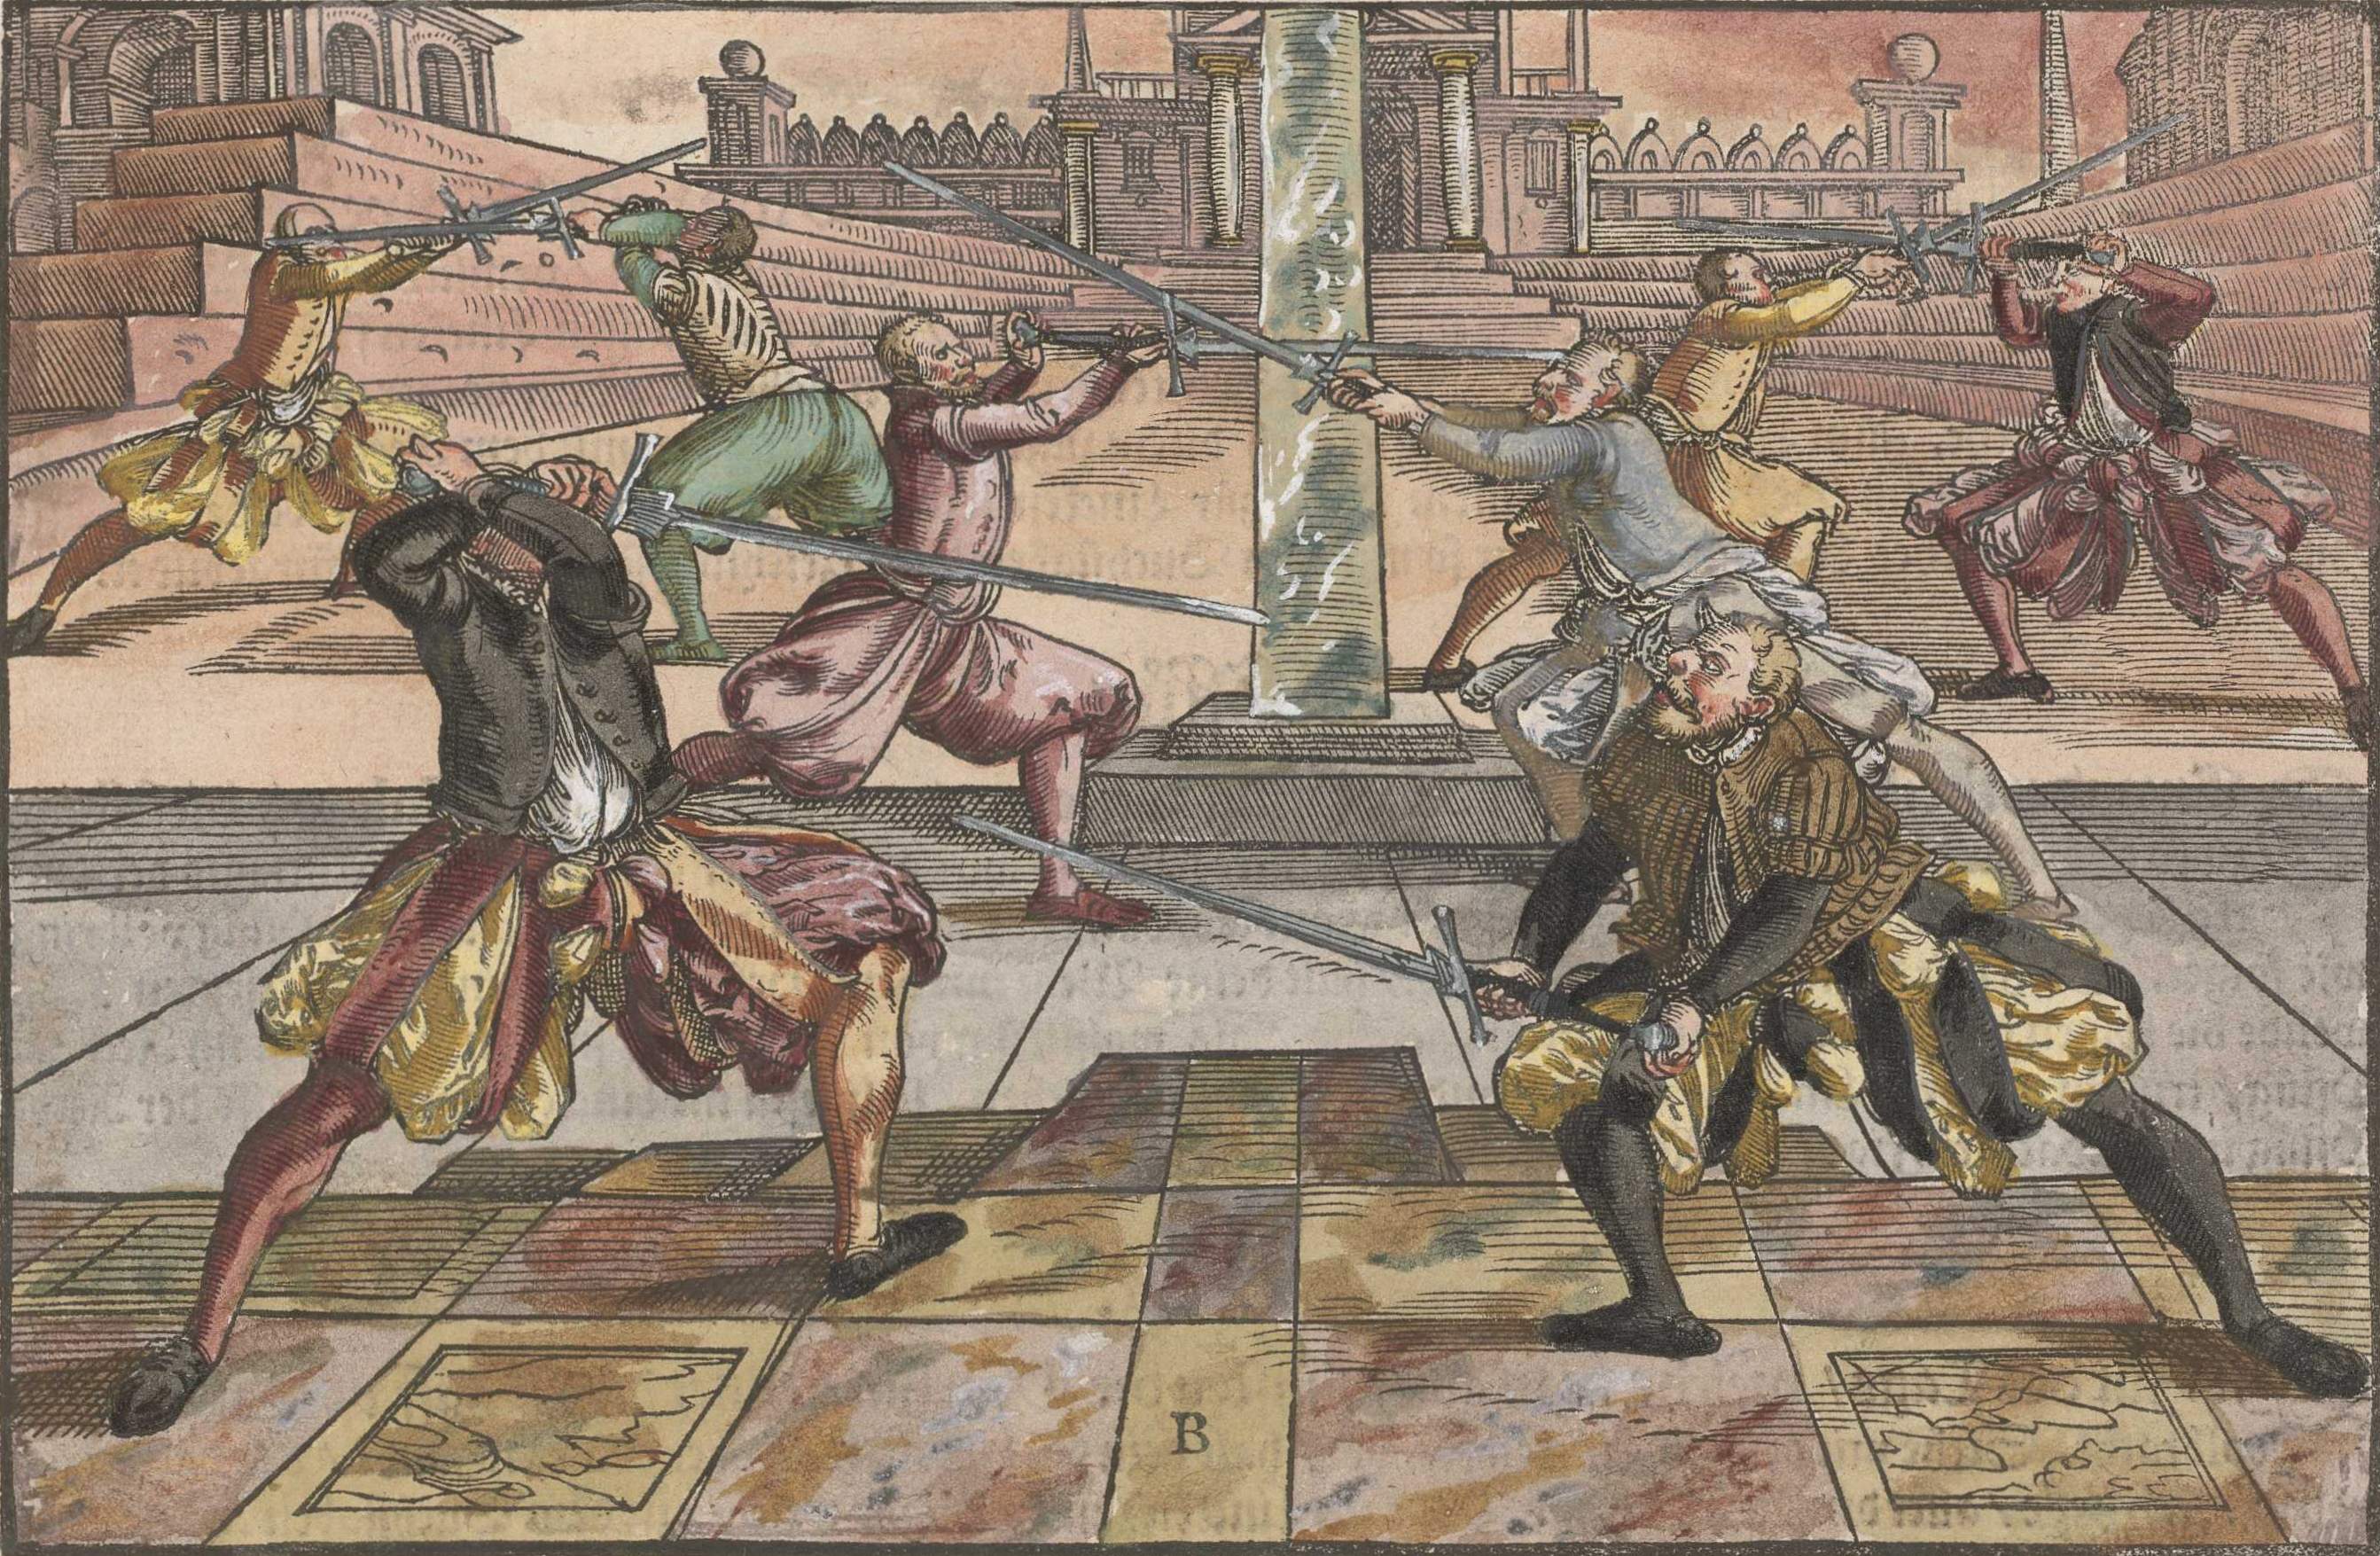
\includegraphics[width=140mm]{../img/Meyer_1570_Sword_B.png}
    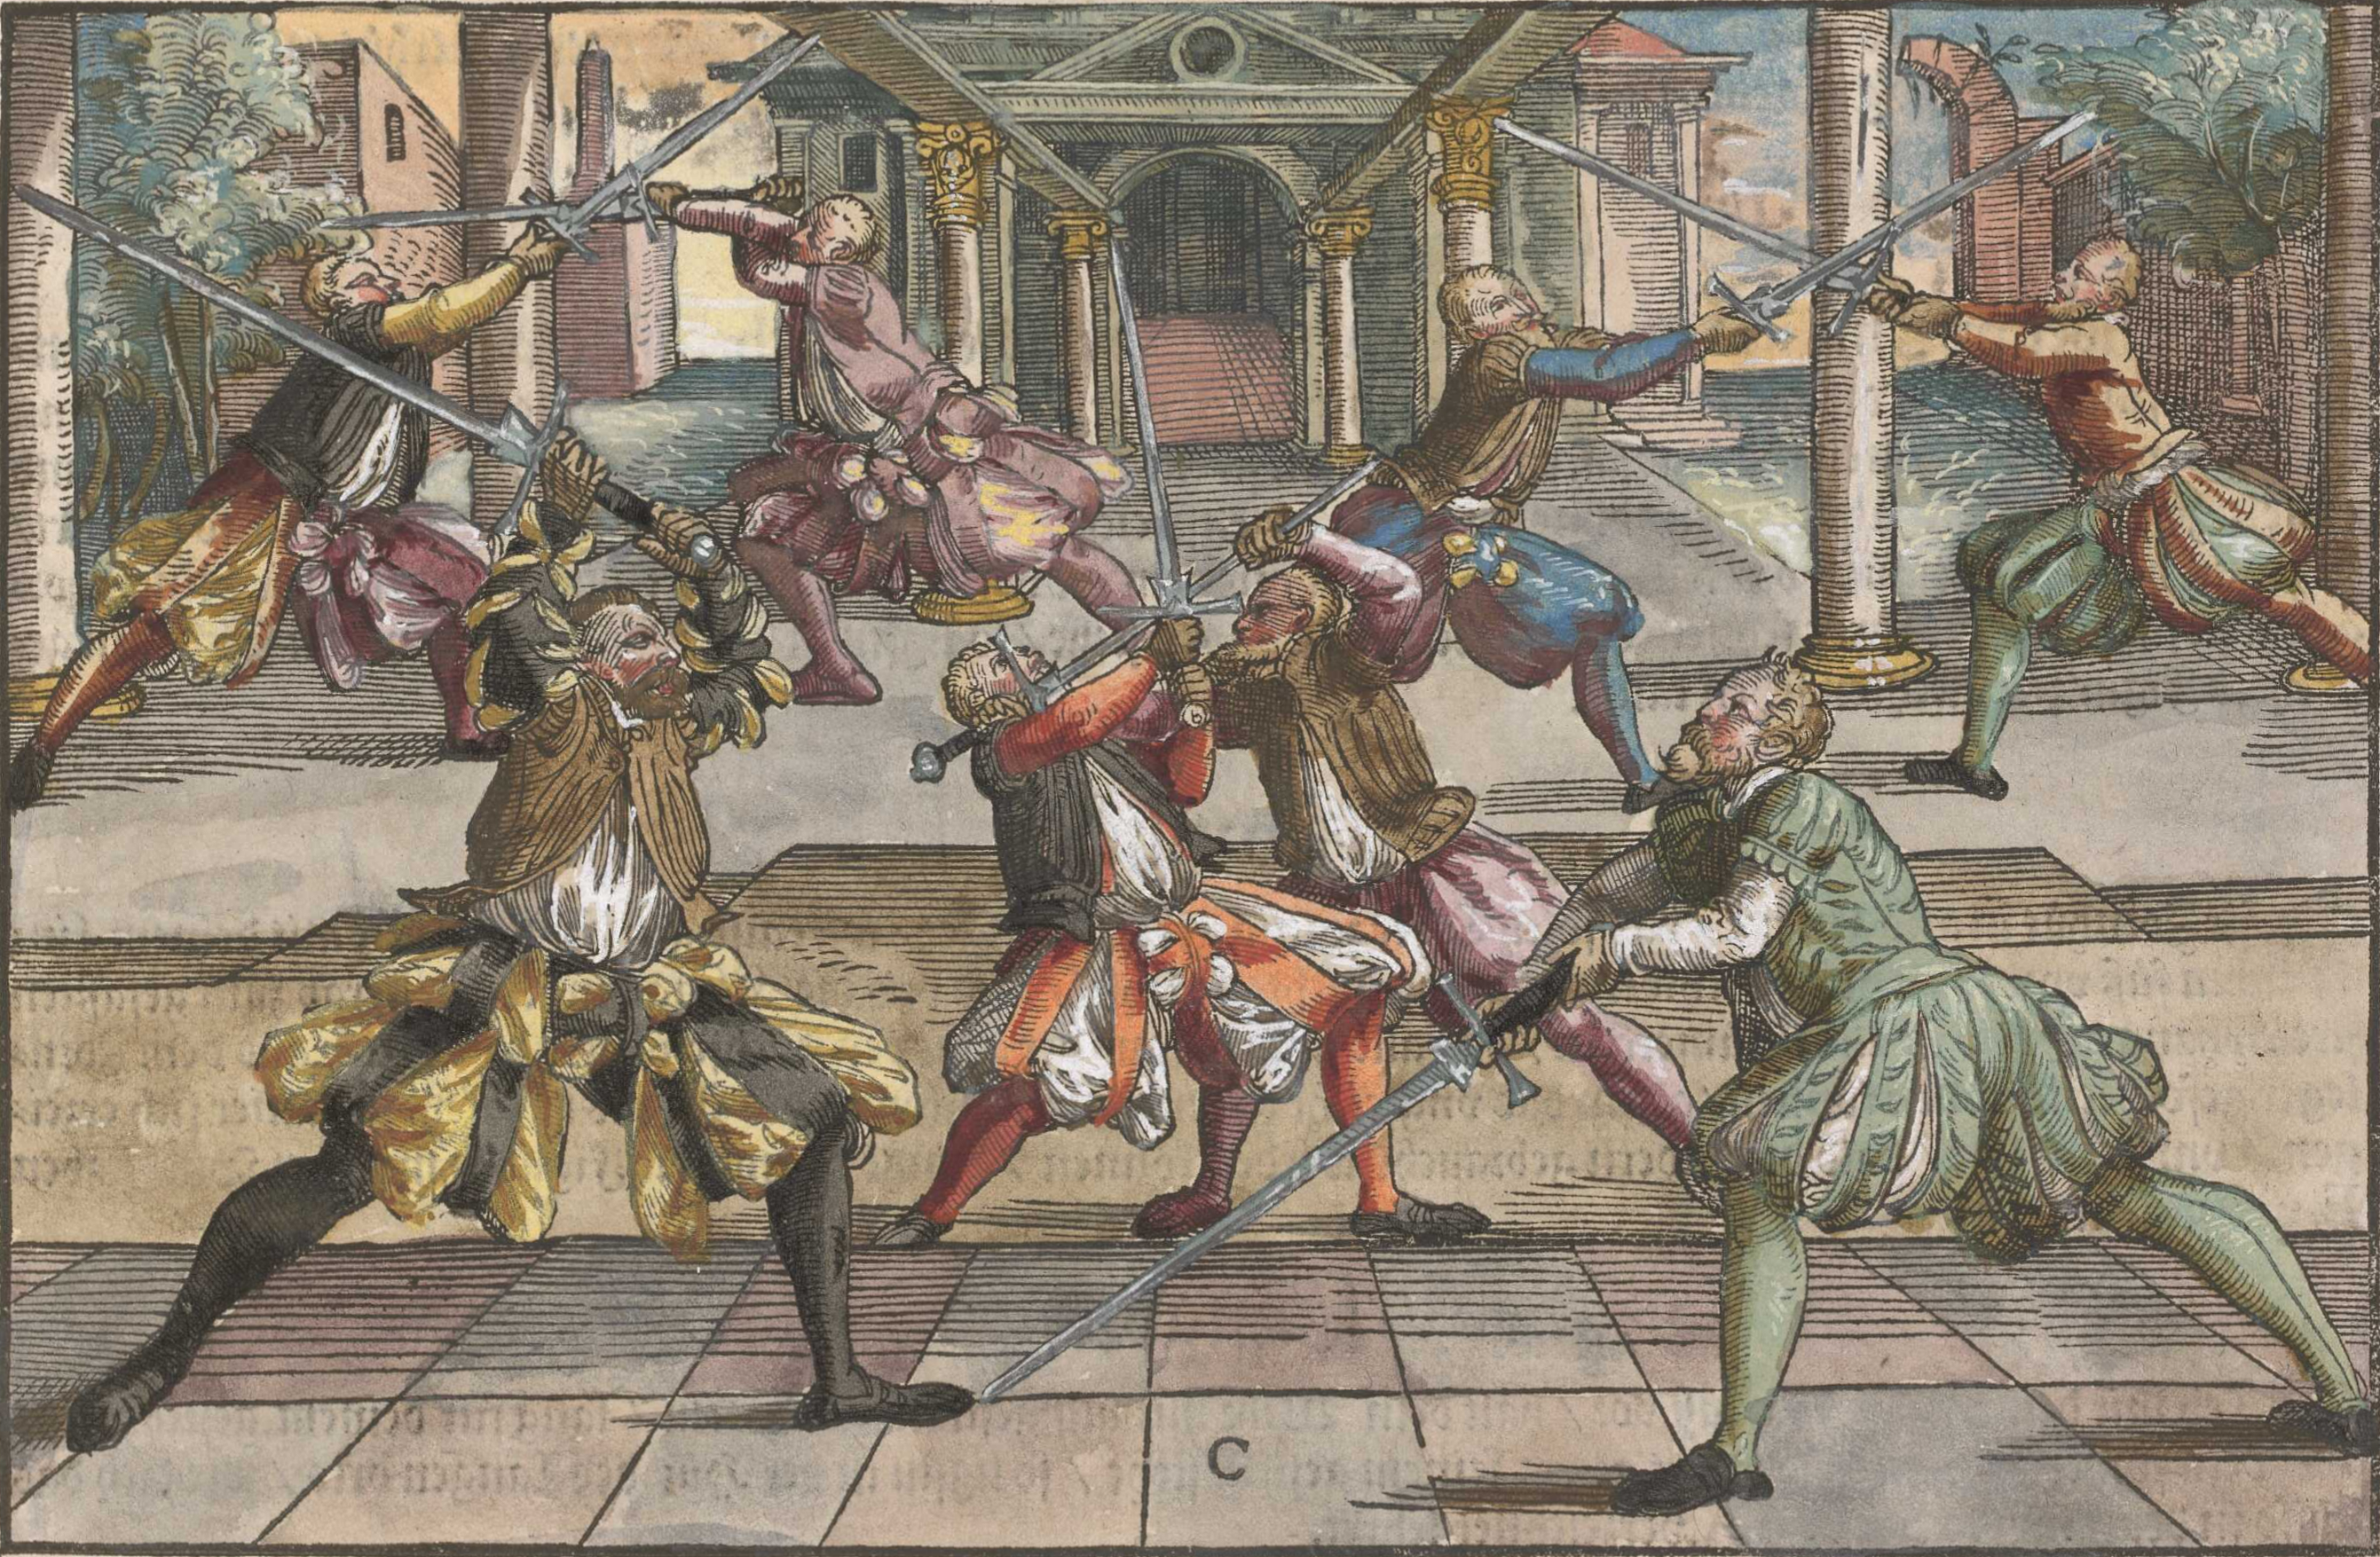
\includegraphics[width=140mm]{../img/Meyer_1570_Sword_C.png}
    \caption{techniky pro jedenapůlruční meč - Joachim Meyer (1570) \cite{KunstDesFechtens}}
    \label{obr01:KunstDesFechtens}
    
\end{figure}

\subsection{Hromadný boj a boj proti přesile}
Souboj jeden na jednoho však může vypadat jako téměř laboratorní podmínky vedle chaotických situací, v rámci kterých v historii běžně k boji docházelo.   

Často se střetávaly větší, více či méně \textbf{organizované skupiny}, případně celé armády čítající mnoho takových pevně ustanovených jednotek. V takové situaci je na místě, aby bojovníkova individualita ustoupila do pozadí - rozhodujícím faktorem je až na výjimky taktické jednání a sladěnost celku. 

Jedním ze základních požadavků, které jsou na vojáka kladeny, je schopnost \textbf{držení formace}. Stojíte-li jako semknutá řada, štít na štít, meče připravené opětovat jakýkoliv úder, který by protivník zkusil na kamaráda vedle, je mnohem těžší prorazit vašimi řadami a dostat se k lučištníkům, kteří nepříteli způsobují těžké ztráty. 

Při skupinové šarvátce hraje zpravidla rozhodující roli taktická \textbf{koordinace} spolubojovníků. Nepřítel, který vám překvapivě vpadl do zad, je mnohem nepříjemnější záležitost, než nepřítel, který postává opodál a čeká, až na něj přijde řada.  

Pro dosažení koordinace je však nutná \textbf{komunikace}. Dohodnout se při šarvátce na postupu, v omezeném čase a aniž by plán byl zachycen protivníkem, vskutku není triviální problém. V kontextu větší bitvy pak důležitost i obtížnost komunikace nabývá zcela nového rozměru a jde o těžký problém, který až do vynálezu moderní vysílačky nebyl uspokojivě vyřešen. Vojenská taktika si vyžaduje flexibilní reakce na změny situace na bojišti, informace musí proudit mezi vojenskými jednotkami a velitelstvím, které jsou často netriviálně fyzicky vzdálené. Jednou možností, jak informaci předat, je vyslání posla - ten je schopen nést detailní informaci, je však zranitelný a pomalý - než dorazí, může již jeho informace být neaktuální. Protipólem pak je broadcast předem dohodnutých signálů, napříkald prostřednictvím trubače - tato cesta je rychlá a v určitém doslechovém okruhu vcelku spolehlivá, avšak signály musí být předem dohodnuté a variant nemůže být mnoho, metoda tedy postrádá flexibilitu a detailnost informace. Jak vidno, jde o zásadní součást vedení bitvy, přesto však vidíme mnoho videoher, které ji zcela zanedbávají.
\bigbreak
Dojde-li k boji \textbf{jediného bojovníka proti přesile}, vše výše uvedené stále platí, akorát očividně kolosální výhody plynoucí z koordinovaného postupu jsou dopřány pouze jedné ze stran. I pro velmi zkušeného šermíře bojujícího proti několika nezkušeným, často jediná šance, jak z takové situace vyváznout, je protivníky rozdělit (kreativním použitím pohybu a znalosti terénu) a zdolat jednoho po druhém rychle, než mu ostatní přijdou na pomoc.

\subsection*{Shrnutí}
Seznámili jsme čtenáře s historickým pozadím a základními prvky, které charakterizují boj s chladnou zbraní v reálném světě. Nyní by měl být připraven pokročit dál a provést srovnání s přístupem, jakým tuto problematiku adaptuje svět videoher.

\clearpage
%------------------------------------------------------------------------------------------------------------------------------------------------------------------------------------------------------------------------------------------------------------%
 % xxxxxxxxxxxxxxxxxxxxxxxxxxxxxxxxxxxxxxxxxxxxxxxxxxxxxxxxxxxxxxxxxxxxxxxxxxxxxxxxxxxxxxxxxxxxxxxxxxxxxxxxxxxxxxxxxxxxxxxxxxxxxxxxxxxxxxxxxxxxxxxxxxxxxxxxxxxxxxxxxxxxxxxxxxxxxxxxxxxxxxxxxxxxxxxxxxxxxxxxxxxxxxxxxxxxxxxxxxxxxxxxxxxxxxxxxxxxxxxxxxxxxxxx %
%------------------------------------------------------------------------------------------------------------------------------------------------------------------------------------------------------------------------------------------------------------%


\section{Chladná zbraň v akčních videohrách}

Nyní, když máme rámcovou představu, jak boj s chladnou zbraní vypadá v reálném světě, nastíníme si, jakým způsobem bývá typicky adaptován v akčních videohrách - jaké jeho aspekty se podařilo v tomto universu věrně zpodobnit, jaké byly ignorovány, a jaké interpretovány s řádnou dávkou umělecké kreativity.

\subsection{Obecný přehled}

Účinkujícími ve hře jsou \textbf{herní postavy}. Ty mohou být ovládané buď hráčem (takovou postavu nazveme \textbf{\acs{PC}}\footnote{\Acl{PC}}), nebo počítačovým algoritmem (tu označíme jako \textbf{\acs{NPC}}\footnote{\Acl{NPC}}), a lze je popsat nějakým jejich \textbf{vnitřním stavem}. Nyní si představíme základní veličiny, které jsou typickou součástí vnitřního stavu postavy ve všech akčních hrách bez ohledu na to, zda jde o hru zaměřenou na boj se střelnou zbraní, chladnou zbraní, či boj jakýkoliv jiný:

\begin{itemize}
    \item \textbf{\ac{HP}}... Číslo udávající zdravotní stav a životaschopnost postavy. \textbf{Pokud klesne na nulu, postava umírá.} K jeho snížení může dojít například úderem protivníkovy zbraně či pádem z výšky a takto odebraným bodům HP říkáme \textbf{\acs{dmg}}\footnote{\Acl{dmg}}. Hráči je stav jeho HP obvykle v reálném čase explicitně komunikován skrze ukazatel na obrazovce. V průběhu boje typicky nejsou doplňovány\footnote{Popřípadě prostředky, skrze které je lze doplnit, jsou vzácné.} a postava musí vystačit s tím, co má - jde tedy o zdroj vybízející k dlouhodobějšímu plánování.
    \item \textbf{Výdrž}... Volitelný avšak častý prvek, číslo reprezentující akutní schopnost postavy vynakládat fyzické úsilí. Spotřebováváno chvatným pohybem a prováděním akcí, v průběhu boje zpravidla dochází k jeho rychlému opakovanému spotřebování a regeneraci.
    \item \textbf{Inventář}... List dalších předmětů, které postava nese s sebou. Může jít o peníze, léčivé lektvary, munici, náhradní zbraně, magické svitky, mapy a cokoliv dalšího v závislosti na hře. 
\end{itemize}

V závislosti na vstupu, který získává od hráče či od řidícího algoritmu, se postava pohybuje po herním světě, interaguje s objekty herního světa a s obsahem svého inventáře a používá svou zbraň. Na použití zbraně se nyní zaměříme.

\textbf{Ovládání zbraně} bývá typicky omezené na stisknutí tlačítka - \textbf{Zaútoč!} - načež postava sama provede útok tak, jak uzná za vhodné - obvykle přehráním jedné ze seznamu animací, které pro danou kombinaci postavy a zbraně předem připravil autor hry.

Implikace, které takto jednoduché rozhraní přináší \textbf{pro hráče}, jsou následující:
\begin{itemize}
    \item \textbf{Intuitivnost} - Hráč, který poprvé spustí hru a zkusí náhodně mačkat tlačítka, rychle ovládání pochopí a začne být ve hře použitelný - žádná nutnost procházet úmorným tutoriálem.
    \item \textbf{Uniformní rozhraní pro všechny zbraně} - Tímto způsobem lze ovládat libovolnou zbraň, ať už jde o dvoumetrovou halapartnu či pěsti hráčovy postavy. Hráč tedy není přehlcen množstvím jednoúčelových herních systémů a z výhod, které získá svým zdokonalováním v použití bojového systému, může těžit po celou hru.
    \item \textbf{Nízká specifičnost} - Rozhraní hráči neumožňuje těžit ze silných stránek žádné konkrétní zbraně. Hra mu skrze bojový systém není schopna poskytnout vzdělávací lekci ohledně vlastností zbraně v reálném světě. Pokud mu tyto vlastnosti již jsou známé, může utrpět jeho imerze.
    \item \textbf{Limitovaná předvídatelnost} - Vzhledem k tomu, že akci, která bude vykonána, nevybírá hráč, ale jeho herní postava, vnáší se tím do hry prvek náhody, který má potenciál hru emocionálně okořenit.\footnote{Pokud však výběr akce probíhá nějakým deterministickým způsobem, hráč v něm brzy intuitivně vypozoruje určité vzory a naučí se akce své postavy do jisté míry předvídat a kalkulovat s nimi při plánování svého postupu - tím může bojový systém získat na hloubce.}
\end{itemize}

A co důsledky, které tento přístup přináší z pohledu \textbf{tvůrce hry}?:
\begin{itemize}
    \item \textbf{Předvídatelnost} - Tvůrce hry má přesnou kontrolu nad tím, jaké akce může jakákoliv postava potenciálně vykonat. Tím se zmenšuje prostor pro výskyt neošetřených okrajových případů.
    \item \textbf{Uniformní rozhraní pro všechny zbraně} - Herní logika, která umí pracovat s jednou zbraní, umí pracovat s každou zbraní. To může dopomoci k celkově čistému a kvalitnímu kódu a značně se tím snižuje námaha s přidáváním dalších zbraní (či jejich procedurální generací za běhu).
    \item \textbf{Nízká specifičnost} - Není možné uspokojivě ztvárnit veškerá zajímavá specifika konkrétní zbraně. Všechny zbraně se musejí chovat do jisté míry podobně. Často je tak zbraň smrštěna do pouhé tabulky statů\footnote{Povrchní veličiny typu dosah, rychlost úderu, míra způsobeného zranění}.
\end{itemize}

Vidíme, že takovéto pojetí boje se zbraní má mnohá pozitiva, stále je však očividné, že \textbf{jde o systém jednoduchý, který sám o sobě nemůže sloužit jako nosná herní mechanika v akční videohře} - oblasti, kde cílová hráčská skupina očekává určitou míru komplexity a hloubky.

Hloubka bývá tomuto systému zpravidla dodávána výběrem mezi několika různými typy útoku (každý efektivní v jiné situaci), akcí pro blokování nepřátelských útoků, důrazem na časování (krátkodobé omráčení nepřítele, navazování úderů, odměna za vyblokování nepřítele v přesně správném okamžiku,...) a \textbf{silným propojením s dalšími mechanikami}, jakými je v první řadě pohyb, dále různé lektvary, magie apod. v závislosti na hře.

Toto si nyní názorně předvedeme na příkladě komerčně úspěšné hry z nedávných let.

\subsection{Zaklínač 3 - vzorový příklad}
Zaklínač 3: Divoký Hon \cite{Wiedzmin3} je akční \acs{RPG} hra, která byla vydána r. 2015 polským studiem CD Projekt. Mezi její hlavní důrazy patří \textbf{otevřený fantasy svět}, propracovaný \textbf{nelineární příběh}\footnote{Hra vychází z knižní série Zaklínač Andrzeje Sapkowského \cite{SapkowskiZaklinac}} a v neposlední řadě také dynamický \textbf{bojový systém}.

Hráč se zde ujímá role Geralta z Rivie - zaklínače, \textbf{profesionálního lovce monster}. Ten je kromě svých dvou mečů\footnote{stříbrného pro boj s nestvůrami a železného proti lidem} vybaven flexibilními možnostmi pohybu, jednoduchými kouzly (tzv. Zaklínačská Znamení) a škálou ručně vařených lektvarů. Na své cestě bojuje s lidmi, duchy, upíry, bazilišky i nepopsatelnými obludami z nočních můr.
Jak tedy vypadají mechaniky, skrze které bylo toto vše umožněno?:


Základem jsou \textbf{dva typy úderů - rychlý a silný}. Jak vyplývá z názvu, rychlý úder je rychlejší, oproti tomu animace silného úderu trvá mírně delší čas, avšak zranění způsobené protivníkovi je také adekvátně zvýšené. K čemu je to dobré? Pro mnoho protivníků platí, že v okamžiku, kdy jim je učiněno nezanedbatelné zranění, přeruší akci, kterou se chystali provádět, a na zlomek času zakolísají. S rychlým úderem je hráč schopen toto zakolísání vyvolat častěji - s dobrým časováním se lze například dostat do cyklu, kdy lehkooděného protivníka hráč udolá jedním úderem za druhým aniž ten se zmohl udělat cokoliv proti vám. Toto stejné zakolísání však může potkat i hráče. Hráč se tedy neustále nachází v časovém tlaku, který ho vybízí kalkulovat - např. zda stihne dva rychlé údery, či raději jen jeden silný, než ho nějaký nepřítel přeruší. Dalším důvodem proč používat silný útok jsou těžkoodění nepřátelé, kterým rychlý útok udílí zranění velmi redukované. 

Drobným doplňkem je akce \textbf{blokování}. Bojujete-li proti lidem, držení tlačítka blokování vás činí prakticky imunním proti běžným útokům mířícím na vás zepředu, za tu velmi drobnou cenu, že sám nemůžete útočit a pohybovat se po bojišti lze jen velmi pomalu. Zajímavější je \textbf{perfektní blokování} - pokud zahájíte blokování přesně v okamžiku, kdy na vás protivník vede úder, provedete odvetný protiúder, který protivníka na pár sekund omráčí. Tím je do boje vnesen další prvek časování. Rovněž je třeba dávat pozor na nepřátele, kteří blokují proti vám.
\bigbreak

Proti chaotickým útokům vedeným změtí zubů a drápů nestvůry však blokování mečem ztrácí smysl. Tehdy přichází na řadu možnosti úskoků a kotoulů, které nabízí \textbf{systém pohybu}. Kromě nich samozřejmě hra nabízí i klasickou chůzi a sprint. Úskok je velmi drobný posun do strany, který nespotřebovává výdrž, pouze má interní cooldown (několik desetin sekundy) zabraňující spamování. Cílem je umožnit hráči tak akorát uskočit z oblasti dopadu nepřítelovy zbraně. Pro zajištění, že tento záměr bude vždy naplněn, je postavě na malý zlomek sekundy poskytnuta celková nezranitelnost. Kotoul je pak rámcově obdobný s tím rozdílem, že spotřebovává výdrž a na oplátku ho lze použít k rychlému překonání velké vzdálenosti. Hra klade velký důraz na hromadné boje, kde hráč musí být schopen prioritizovat cíle a rychle využívat objevivších se zranitelností jednotlivých nepřátel. Vysoká mobilita, kterou kotoul poskytuje, je tedy více než nápomocná.  

Zaklínačská Znamení do boje přinášejí další vrstvu komplexity. Jde o \textbf{5 kouzel}, která spotřebovávají velkou porci výdrže a na oplátku zaklínači mocně pomohou - např. může jít o ochranné silové pole, poryv větru, který má šanci omráčit zasažené protivníky, či zmatení, které přiměje nepřítele bojovat na vaší straně.

Výčet Znamení je pevně stanoven, avšak klasicky pro žánr \acs{RPG}, hra zahrnuje \textbf{prvky progrese}, pomocí kterých lze Znamení v průběhu hry vylepšovat a modifikovat. Stejné platí i pro boj s mečem - rychlý i silný úder mají každý své vlastní stromy dovedností, které jsou schopny zajímavými způsoby ovlivnit gameplay. 

Poslední částí zaklínačova repertoáru, kterou zmíníme, jsou lektvary a oleje. Jde o \textbf{konzumovatelné předměty}, které hráč v průběhu hry sám vyrábí, a po jejich konzumaci (požití lektvaru postavou / namazání oleje na meč) mu je na určitý časový limit poskytnut nějaký bonus (př. regenerace zdraví, bonusové zranění proti upírům apod.). Jde tedy o zdroje, se kterými hráč hospodaří v dlouhodobějším horizontu, ale použity v kritickém okamžiku mohou zvrátit výsledek boje. 

Esenciální součástí každé hry s bojovými prvky, jsou také \textbf{nepřátelé}. V této oblasti byl Zaklínač 3 k hráči velmi štědrý. Najdeme zde obyčejné lidské nepřátele (bandity, nepřátelské vojáky apod.), jejichž způsob boje sdílí mnoho prvků se zaklínačovým - např. jsou schopni blokovat jeho údery. Dále pak širokou paletu monster všech velikostí a tvarů, pozemní i schopné létat vzduchem, vybuchující, duchy zranitelné pouze specifickými cestami, tvory vládnoucí magií - každý nepřítel má své osobité silné a slabé stránky a vybízí hráče k jinému stylu hraní.

\bigbreak

Vidíme, že bojový systém Zaklínače 3 je zjevně postaven kolem kostry, kterou jsme si načrtli v předchozí kapitole, zároveň jde o systém mající značnou hloubku. Tato hloubka je získána z velké části důrazem na celkový hráčův přehled o situaci na bojišti, škálou osobitých nepřátel, důrazem na časování, a pak také propojením s dalšími systémy - pohybem, magií a vařením lektvarů. 

Hráči je poskytnut prostor k budování dovednosti a k důmyslnému taktizování jak v krátkodobém, tak v dlouhodobém horizontu. Celkové kvality bojového systému ostatně potvrzuje značný komerční úspěch, kterého se hře po vydání dostalo.

Mezi možné příčiny úspěchu hry můžeme zařadit také pozorování, že \textbf{hloubka systému je volitelná}. Rekreační hráč, který hraje převážně kvůli příběhu, si ji může dovolit víceméně ignorovat. Stačí hru nastavit na nízkou obtížnost a většinu nepřátel není těžké udolat pouze s povrchní znalostí základních mechanik. Není odvážné tvrdit, že to může mít pozitivní vliv na velikost cílového hráčského publika. 

\subsection{Chladná zbraň jako doplňkový prvek}

Chladnou zbraň najdeme také v mnoha hrách, ve kterých není stěžejním prvkem. Například ve většině her žánru \textbf{\acs{FPS}} najdeme kromě širokého výběru palných zbraní i nějaký nůž jako poslední zálohu když dojde munice, v žánru \textbf{stealth} často vidíme chladnou zbraň jako prostředek k tiché likvidaci nepřátel a takto bychom mohli pokračovat. Mnohdy taková zbraň odpovídá popisu z 1.2.1 - cílem není, aby chladná zbraň sama o sobě byla zajímavou mechanikou, naopak \textbf{tvoří pouze jeden dílek} ve skládačce herního systému a pro hráče musí především být jednoduše uchopitelná. 

Přesto najdeme mnoho takových zbraní, které se staly \textbf{ikonickým symbolem} své hry - zmínit můžeme například hru DOOM \cite{DOOM1993} a motorovou pilu, či páčidlo ze série Half-Life \cite{HalfLife}.


%------------------------------------------------------------------------------------------------------------------------------------------------------------------------------------------------------------------------------------------------------------%
 % xxxxxxxxxxxxxxxxxxxxxxxxxxxxxxxxxxxxxxxxxxxxxxxxxxxxxxxxxxxxxxxxxxxxxxxxxxxxxxxxxxxxxxxxxxxxxxxxxxxxxxxxxxxxxxxxxxxxxxxxxxxxxxxxxxxxxxxxxxxxxxxxxxxxxxxxxxxxxxxxxxxxxxxxxxxxxxxxxxxxxxxxxxxxxxxxxxxxxxxxxxxxxxxxxxxxxxxxxxxxxxxxxxxxxxxxxxxxxxxxxxxxxxxx %
%------------------------------------------------------------------------------------------------------------------------------------------------------------------------------------------------------------------------------------------------------------%



\section{Hry s větší kontrolou}

Nyní víme, jakým způsobem je typicky chladná zbraň v akčních hrách ztvárňována, známe pozitiva, která tato cesta přináší, a rovněž některé triky, jak jejím prostřednictvím dosáhnout poutavého bojového systému. Co nás ale čeká, kdybychom chtěli sejít z vyšlapané cesty a nabídnout hráči nad jeho zbraní větší míru kontroly?

\subsection{Benefity a výzvy}

Neprve se zamysleme, \textbf{proč by hráč o větší kontrolu mohl mít zájem}:
\begin{itemize}
    \item \textbf{Je to poučné} - Jedním z hlavních cílů videoher celkově je zprostředkování zážitku, který je pro hráče z různých důvodů nedosažitelný v reálném světě. Skrze hru, která mu zprostředkuje přímou kontrolu nad mečem, může hráč získat větší pochopení k problematice historického vedení boje.
    \item \textbf{Šerm ho baví v reálném světě} - Naopak, hráč může být aktivním šermířem, avšak chce si zážitek z boje užít ve zjednodušené podobě i v pohodlí domova.
    \item \textbf{Nemá rád když ho hra omezuje} - Nemalá skupina hráčů si ráda hledá vlastní cestu hrou a vyžaduje od hry plnou svobodu v tom, co jim je umožněno dělat. 
    \item \textbf{Chce zkusit něco nového} - Mnoho hráčů se již zkrátka nudí z donekonečna omýlaného klišé, jakým se v jejich očích boj s chladnou zbraní stal - líbí se jim téma, ale zároveň ho chtějí zkusit pojaté neotřelým způsobem.
\end{itemize}

Dále, jaké benefity by takový přístup mohl přinést \textbf{tvůrci hry}:
\begin{itemize}
    \item \textbf{Emergentní gameplay} - Tvůrci hry stačí, aby zprovoznil robustní systém, který hráči umožní obecný pohyb meče. Najít zajímavou metodiku jak systém použít, je již úkolem hráčské komunity. Takto může dojít k živelnému objevení mechanik, které tvůrce hry nikdy ani neplánoval, čímž hra může být značně obohacena.  
    \item \textbf{Nástroj interakce s okolním prostředím} - Pohybem meče v 3D prostoru se dá zprostředkovat široká škála interakcí s okolním prostředím, které by jinak musely být implementovány odděleně (zmíníme např. mačkání tlačítek či páčení víka truhlice). Také se tím otevírá cesta pro zcela nové interakce, které se s použitím meče jeví přirozené, bez něj by však bylo těžké najít cestu, jak je do hry zakomponovat (např. odrážení střel, srážení hledí protivníkovy přilby, odpalování předmětů na protivníka apod) .   
\end{itemize}

Vidíme, že motivace k umožnění větší kontroly je silně nezanedbatelná. Očividně tedy takovým pokusům musí stát v cestě výrazné překážky vzhledem k tomu, že víme, že se jim dosud nepodařilo ovládnout herní mainstream.

\textbf{Jaké očividné problémy je tedy třeba vyřešit?}
\bigbreak
Prvním je \textbf{ovládání}. Meč je obecný objekt v 3D prostoru, má tři stupně volnosti pro polohu a další tři pro rotaci. Nemluvě o dalších vlastnostech - např. jak pevně ho šermíř drží. Pro žádnou z těchto veličin se nenabízí očividný způsob, jak ji zanedbat či odvozodit z těch ostatních. Abychom mohli mečem sekat, bodat a blokovat údery, potřebujeme pohybovat rukojetí a natáčet čepel, obojí po všech třech osách. Rotace meče kolem jeho středové osy by se zdála jako vhodný kandidát k implicitnímu odvozování, avšak např. k odpalování projektilů je velmi vhodné moci zajistit, že do nich udeříme plohou stranou meče, místo abychom je rozsekli ostrou hranou čepele.

Oproti tomu \textbf{počítačové periferie}, které se běžně používají jako zdroj hráčského vstupu - tedy myš a klávesnice, popřípadě ovladače u herní konzole - poskytují informaci nanejvýše dvourozměrnou (horizontální a vertikální osa). Neexistuje tedy přímočarý a intuitivní způsob, jak na ně pohyb meče namapovat - je nutné učinit kompromis a nějakým způsobem volnost pohybu meče omezit. Alternativní metody ovládání, které tento problém nemají, existují, a stručně se na ně podíváme později v této kapitole, jejich rozšířenost mezi hráči však není taková, aby bylo rozumné spoléhat, že jimi naše cílová skupina disponuje.
\bigbreak
Pokud se nám podaří problém ovládání uspokojivě vyřešit, narazíme na další v oblasti \textbf{hratelnosti}. Důležitou součástí dynamiky boje s chladnou zbraní je předvídání protivníkových úderů a reagování na ně ještě dříve, než se stanou. V reálném světě je šermíř schopen pozorovat drobné pohyby svalů a očí protivníka, které v tomto ohledu mnohé napoví. V počítačové hře samozřejmě je hráčova schopnost vnímat takovéto detaily velmi omezená. Tento problém je ve hrách typicky řešen tak, že animace úderů zahrnují jako počáteční fázi výrazný nápřah. Jak však zajistíme takovéto výrazné telegrafování útoků, pokud má nepřítel nad mečem jemnou kontrolu a může z principu věci dělat co si jen zachce? Chceme vůbec ve hře mít výrazné telegrafování vzhledem k tomu, že neodpovídá realitě? Rozlousknutí tohoto problému si vyžaduje kompromisy.
\bigbreak
V neposlední řadě, plná kontrola nad mečem nemusí vhodně ladit s \textbf{narativní} složkou hry. V mnoha akčních hrách prezentuje příběh hráčovu postavu jako zkušeného šermíře, ne-li přímo virtuosa meče, jakému se v herním světě vyrovná jen hrstka dalších. Problémem však je, že většinový hráč srovnatelně zkušeným šermířem s největší pravděpodobností není. Je-li šermířská dovednost postavy fakticky přímo úměrná hráčově dovednosti, může tím tedy docházet k narativní disonanci. Zahrnutím takového bojového systému se designérům, kteří mají narativ na starosti, citelně komplikuje práce. 
\bigbreak
Finálně, pokud jsme všechny tyto problémy vyřešili, čeká nás implementace systému. Hráči jsme nabídli v podstatě neomezené možnosti, nabízí se tedy otázka, jakým způsobem se hodláme ujistit, že možnosti skutečně neomezené jsou a nevyskytly se nějaké \textbf{neočekávané okrajové případy}, které nebyly ošetřeny a povedou k nedefinovanému chování? Jednou z cest je přeci jen kontrolu nad mečem omezit a smrsknout ji na stále velkou, avšak \textbf{konečnou množinu stavů}, které jsou tvůrci schopni projít jednu po druhé a ujistit se, že každý funguje, jak zamýšleli. Jedinou další alternativou se zdá být \textbf{plně realistická fyzikální simulace meče} - problémům, které tato cesta přináší, je věnována převážná část této práce.  
\bigbreak
Vidíme, že poskytnout hráči přímou kontrolu nad mečem, je nevděčný úkol vyžadující mnoho kompromisů. V historii najdeme pouze několik her, které se s ním pokusily popasovat, každá svým unikátním způsobem. Na ty se nyní podíváme blíže.

\subsection{Die by the Sword}

Průkopníkem v této oblasti je Die by the Sword \cite{DieByTheSword}, hra vydaná kalifornskou společností Treyarch Corporation roku 1998. 

Jde o jedinou hru, kterou si zde představíme, jež se nevydala cestou omezení množiny stavů meče na konečné množství, ale nabídla hráči skutečně \textbf{jemnou, spojitou kontrolu}. Ta byla umožněna zapojením jednoduchého \textbf{realistického fyzikálního subsystému}, což byl na tehdejší dobu úkaz vskutku nevídaný vzhledem k hardwarovým omezením, v jejichž rámci bylo nutno operovat.

\textbf{Backend hry} umožňoval \textbf{plně volný pohyb} všech objektů třímaných herní postavou (postava mohla např. v jedné ruce držet meč a ve druhé štít či druhý meč), přičemž tělo postavy bylo \textbf{procedurálně animováno} (další na tuto dobu vzácný úkaz), aby poloha jejích rukou s polohou objektů korespondovala.

Tento přístup k implementaci přinesl některé \textbf{zajímavé důsledky}. Hráč se nemusel učit používat dedikovanou mechaniku pro blokování nepřátelských úderů, stačilo meč napolohovat tak, aby tomu nepřátelskému stál v cestě. Podobným způsobem zde byl nepřeberný prostor pro další zajímavé techniky, vyvíjené a zdokonalované plně hráčskou komunitou. Dále, díky obecnosti systému nebyl problém mít nepřátele všech představitelných tvarů a velikostí - dokud měl nepřítel hmotné tělo, mohli jste ho mečem trefit; dokud měl nějakou končetinu, mohl sám držet zbraň. Spojením se systémem procedurální animace nestvůrám bylo možné velmi efektně odsekávat kusy těla a kochat se jejich zvýšenou nemotorností\footnote{případně rovnou neschopností hráče zranit, pokud byla odseknuta končetina třímající zbraň}. K dovršení dojmu vás hra nechala chopit se odseknuté končetiny jako zbraně, stále při stejném ovládání, jaké vám nabídl meč.

Kamenem úrazu pro hru však nesporně bylo \textbf{ovládání}. Tvůrci hry si byli zřejmě vědomi, o jak náročnou výzvu vyžadující dlouhodobý výzkum v případě této hry jde, a nabídli hned několik velmi odlišných metod vstupu pro udání pohybu zbraně:
\begin{itemize}
    \item \textbf{Numerická klávesnice}\footnote{V době vzniku hry nebyl grafický operační systém ovládaný myší běžnou součástí výbavy každého hráče. Od her se očekávalo, že budou podporovat možnost ovládání čistě pomocí klávesnice.} - Obdélník číselných kláves symbolizoval obdélník obrazovky, stisknutí dvou kláves (poloh na obrazovce) v rychlém sledu znamenalo švih mečem z jedné polohy na druhou.
    \item \textbf{Myš} - Myší bylo možné udávat pohyb spojitým způsobem. Poloha kurzoru na obrazovce se mapovala na polohu v herním světě, kam se má švihem meč přesunout. 
    \item \textbf{Nahrávky} - Ve hře byl obsažen dedikovaný nástroj umožňující pomocí časové osy a klíčových snímků - způsobem známým z profesionálního softwaru pro tvorbu animací - vytvářet a editovat vlastní zcela libovolné pohyby zbraně. Hotové nahrávce bylo následně možné přiřadit klávesu, jejímž stisknutím ji postava ve hře přehrála. 
\end{itemize}   
Přes značné úsilí, které tvůrci této oblasti věnovali, stalo se ovládání hlavním předmětem hráčské kritiky. Mnoho hráčů si stěžovalo, že je hra jeho vinou nadmíru těžká, případně že si zkrátka \textbf{nehodlají na neotřelý způsob ovládání zvykat}. Přestože hra byla značně oceněna profesionálními kritiky, mezi širokou herní veřejností se jí výrazných ohlasů nedostalo. Kromě datadisku Limb from Limb se již na její odkaz žádná další hra nepokusila navázat, pokud je autorovi této práce známo.

\bigbreak
Celkově vidíme, že hra přinesla systém poskytující \textbf{dodnes nepřekonanou flexibilitu}, nemající problém s nepřáteli všech tvarů, sofistikovanou interakcí s prostředím a umožňující vydatnou dávku emergentního gameplaye. Kamenem úrazu se jí však stalo ovládání. Celkově hra ukázala, že \textbf{návrh ovládání} pro takto flexibilní systém \textbf{je těžký problém}, který vyžaduje více výzkumu.

\subsection{Mount\&Blade}

Kultovní klasikou je Mount\&Blade \cite{MountAndBlade}. První verzi této hry vydalo turecké studio TaleWorlds v roce 2008, později se hra pro velkou oblíbenost mezi hráči dočkala datadisku Warband a velmi nedávno i druhého dílu Bannerlord, který mnoho mechanik hrubě nastíněných v původní hře dále rozvádí a prohlubuje. My se zde budeme věnovat prvnímu dílu, který je v kombinaci s datadiskem Warband i v dnešní době mezi hráči velmi oblíbený a materiálů pro analýzu nám poskytne zcela dostatečné množství.

Jde o \textbf{sandbox} s \acs{RPG} prvky, kde se hráč ujímá role vůdce žoldnéřské skupiny. V jeho kůži putuje od království ke království, verbuje vojáky, plní úkoly pro okolní šlechtice a účastní se po jejich boku bitev se šlechtici znepřátelených zemí. Svět je velmi silně inspirován středověkou Evropou, nenajdeme zde žádnou magii. Nepřáteli jsou výhradně lidé. 

Ovládání vlastní hráčské postavy zde tvoří pouze polovinu skládačky bojového systému - tou druhou je udílení rozkazů zverbovaným vojákům. V bitvách se zde střetávají typicky vyšší desítky až nižší stovky bojovníků spřátelených a nepřátelských. \textbf{Hráčská postava je zde pouze jedním z mnoha} - počítačem řízení bojovníci mají shodné možnosti pohybu i ovládání zbraně a podléhají stejnému systému \acs{RPG} progrese. 

Jak tedy vypadá ovládání zbraně? Každá zbraň má definovanou \textbf{množinu útoků}, které lze provádět. Hráč stiskem tlačítka myši zahájí nápřah, dle polohy kurzoru je vybráno, který z útoků bude vykonán (např. nápřah nad hlavou kurzorem uprostřed nahoře, bodnutí kurzorem uprostřed obrazovky apod.), následně uvolněním tlačítka myši je útok vykonán.

Zbraní najdeme více druhů - meče, sekery, kyje, kopí a další. Útočné zóny jsou napříč zbraněmi shodné, pouze \textbf{některé zóny u některých zbraní chybí} (meč poskytuje všechny, kyj neumožňuje bodání, s kopím lze pouze bodat apod.). Animace, která se přehraje pro útok v dané zóně, je však unikátní pro daný typ zbraně\footnote{Nedochází k žádnému náhodnému výběru, danému páru \textit{zbraň - útočná zóna} přísluší vždy právě jedna pevně daná animace.}.

Druhým typem akce, který lze vykonávat, je \textbf{blokování}. Je-li hráč vybaven štítem, stačí držet stisknuté levé tlačítko myši a postava je kryta proti veškerým úderům, které na ni míří zepředu. Chce-li však postava provést útok se zbraní, musí nejprve kryt přerušit, čímž ochrany pozbyde. Dalším omezujícím faktorem je omezená odolnost štítu - utrží-li štít určité množství \acs{dmg}, je zničen a postava ho zahodí. Čímž přijde na řadu obtížnější situace - blokování pomocí zbraně. Zde se opět dostáváme k využití úderových zón - zkrátka zóna, ve které obránce blokuje, musí odpovídat zóně útočníka - jinak k vyblokování úderu nedojde.

Prvkem, který umocňuje hráčův dojem realističnosti, je \textbf{výpočet zranění}. Hra se obecně nepokouší o realistickou fyzikální simulaci, avšak způsobené zranění je přesto determinováno kombinací mnoha faktorů, které realistické chování účinně aproximují - zmíníme rychlost zbraně, délku její dráhy apod. . Dále je využíváno jemné detekce kolizí. Zaprvé k tomu, aby se určila zasažená část těla - různým částem těla postavy odpovídá různý kus zbroje, která určuje, jakou mírou má zranění být redukováno. Zadruhé, zranění je velmi silně redukováno, pokud při své cestě zbraň prošla skrze zeď či jiný prvek okolního prostředí. 

Nyní rámcově víme, jak bojový systém funguje. Pojďme se tedy podívat na benefity, které z této implementace plynou. Vidíme, že hře se \textbf{podařilo najít kompromis} slučující některé prvky, které by se z naší předchozí anylýzy mohly zdát vzájemně protichůdné.
\begin{itemize}
    \item \textbf{Jednoduchost X Pocit kontroly} - Hráčova kontrola nad mečem je sice omezená na výběr z malé množiny úderových zón, těch je však stále dostatečné množství, aby pokryly většinu způsobů útoku, které by běžnému hráči rozumně mohly přijít na mysl. Protože správný výběr útoku má velmi reálný efekt na jeho úspěch, hráč je motivován svou možnost volby vzít plně na vědomí a ne ji přejít jako pouhý kosmetický detail. 
    \item \textbf{Uniformní ovládání X Osobitost jednotlivých zbraní} - Ovládání odpovídá napříč zbraněmi totožné šabloně, konkrétní provedení vyžádaného útoku se však mezi typy zbraní liší dostatečně, aby to mělo citelný efekt na pocit ze hry. Rovněž fakt, že pro každý pár \textit{zbraň - typ útoku} existuje pouze jediná pevně daná animace, umocňuje předvídatelnost, která hráči umožňuje zbraň rychle pochopit a být si intuitivně vědom jejích specifik.
\end{itemize}

Systém však přinesl i některá nepohodlí a promarněné příležitosti:
\begin{itemize}
    \item \textbf{Ovládání kamery} - Pohyb myši plní současně dvě nesouvisející role - ovládání natočení kamery a výběr zóny útoku - což se ne vždy dobře slučuje. Nastávají situace, kdy hráč, aby vybral směr útoku, musí pohled přetočit pryč z místa zasluhujícího pozornost, což může vést k mírnému zmatení.  
    \item \textbf{Emergentní gameplay} - Bojový systém je uzavřená bublina, která s okolními mechanikami ani sama se sebou neinteraguje natolik, aby vznikl prostor pro vznik zajímavých interakcí, jaké tvůrci hry úmyslně neplánovali.
    \item \textbf{Flexibilita} - Do hry by bylo obtížné přidat např. specifický typ nehumanoidních postav - celý systém útočných zón by se musel překopat, aby byl boj s nimi schopen poskytnou stejně realistický zážitek jako boj s lidmi.
\end{itemize}

Celkově tedy vidíme, že hře se podařilo najít \textbf{zajímavý kompromis mezi realističností, pocitem kontroly, a hráčskou přívětivostí}. O jeho kvalitách svědčí dlouhodobě velmi pozitivní ohlasy hráčské komunity. Bylo toho však dosaženo obětováním jisté vnitřní flexibility - systém velmi dobře vystihuje boj lidí s lidmi, použití zbraně k jakémukoliv jinému účelu by však žádalo jeho významné překopání. 


\subsection{Kingdom Come: Deliverance}
Poslední hrou, kterou zmíníme, je Kingdom Come: Deliverance \cite{KCD}, vydáné roku 2018 českými Warhorse Studios. Jde o akční \acs{RPG} odehrávající se v českém Posázaví roku 1403. Jedním z hlavních důrazů hry byla historická věrnost a celková realističnost zážitku - z tohoto rozhodnutí plynou přirozeně dalekosáhlé důsledky pro bojový systém.

Ústřední myšlenka je zde podobná jako u Mount\&Blade, s tím rozdílem, že na její implementaci bylo věnováno \textbf{řádově více zdrojů a lidského úsilí}. Najdeme zde velmi podobný systém zón útoku, mezi kterými hráč vybírá pohybem kurzoru, tvůrci zde však vytvořili tisíce dílčích animací, které jsou skládány do naprosto realisticky působícího pohybu zbraně i šermíře. Systém byl vyvíjen na základě konzultace s odborníky na středověký způsob boje, animace tedy i odpovídají skutečným historickým technikám. Dále systém zahrnuje neznámý avšak pravděpodobně značný počet rozličných heuristik, které se pro hráče neviditelným způsobem starají o vyšší responzivitu, další realističnost atd. .

Celkově jde o systém nabízející značnou hloubku. Najdeme zde například propracovaný systém komb, velký důraz na správu výdrže a časovací události pro blokování nepřátelských úderů. Hráčské ohlasy dávají za pravdu, že hra nabízí \textbf{nejrealističtější zážitek boje s chladnou zbraní, jaký najdeme na trhu}.

Pokoušet se zde o hloubkový rozbor však nemá valný smysl - byl by to úkol obtížný a jeho splnění by nám nepřineslo mnoho užitku, protože napodobení jakéhokoliv jednoho dílčího aspektu takového bojového systému se naprosto \textbf{vymyká časovým i finančním možnostem autora této práce}.


\section{Alternativní ovladače}

(představení - ovladače co mohou být pro náš účel ovládání meče víc vhodné - existují ovladače co se postupně dostávají do mainstreamu, co jsou state-of-the art ve svém obskurním niche oboru, i naprosto experimentální ovladače co jsou teprve předmětem výzkumu)

\subsection{Virtuální realita}

(jaké má výhody)

(příklad hry kde se s ním ovládá meč) (swords\&sorcery, gorn, beatsaber)

(nevýhody)
- disonance "meč narazil do něčeho a není tam kde ovladač"

(proč se jí nebudeme při výzkumu zabývat)
- pořád není mainstream
- (zjistit) uzavřenost platforem?


\subsection{Pohybové senzory ve smartphonu}

(výhody)
- dostupnost
- otevřenost platformy, programátorská flexibilita (hackovatelnost)

(nevýhody)
- fragmentace mobilního trhu, nekonzistence výstupu senzorů mezi různými mobily
- způsob připojení (ne každej desktop má bluetooth nebo wifi, kabel je nepraktickej; celkově mobily asi maj problém s nízkolatenčním přenosem po místní síti)
- najít nějakej článek

\subsection{Obskurní periferie}

3d myš
- extrémně drahá 
- stavěná pro 3d modelováni
- nemá 6 ale jenom 3 stupně volnosti


\section{Shrnutí}

%%% Fiktivní kapitola s ukázkami citací

\chapter{Odkazy na literaturu}

Odkazy na literaturu vytváříme nejlépe pomocí příkazů
\verb|\citet|, \verb|\citep| atp.
(viz {\LaTeX}ový balíček \textsf{natbib}) a~následného použití
Bib{\TeX}u. V~matematickém textu obvykle odkazujeme stylem \uv{Jméno
autora/autorů (rok vydání)}, resp. \uv{Jméno autora/autorů [číslo
odkazu]}. V~českém/slovenském textu je potřeba se navíc vypořádat
s~nutností skloňovat jméno autora, respektive přechylovat jméno
autorky. Je potřeba mít na paměti, že standardní příkazy
\verb|\citet|, \verb|\citep|
produkují referenci se jménem autora/autorů v~prvním pádě a~jména
autorek jsou nepřechýlena.

Pokud nepoužíváme bib\TeX{}, řídíme se normou ISO 690 a zvyklostmi
oboru.

Jména časopisů lze uvádět zkráceně, ale pouze v~kodifikované podobě.
%%% Fiktivní kapitola s ukázkami tabulek, obrázků a kódu

\chapter{Schéma ovládání}
\chapter{Implementace}

\section{Návrh systému}

\subsection{Stručný celkový přehled}

- šermíř.. rigidbody
  meč.. další rigidbody připojené jointem

(insert uml diagram here)
- SwordMovement, SwordsmanMovement a související komponenty (možná rozdělit do 2 diagramů?)


\subsection{Zpracování uživatelského vstupu}

\subsection{Mody ovládání}

\subsection{Animace šermíře}

\subsection{Počítání zranění}


\section{Stabilita simulace}

\subsection{Jak nastavit cílovou rotaci jointu}

\subsection{Ladění parametrů}

\subsection{Kolize mečů}


\section{Shrnutí}

\chapter{Implementace}

V předchozí kapitole jsme navrhli strukturu, které se náš projekt bude držet. Stejně tak již víme, jakým způsobem bude se systémem interagovat hráč. Nyní můžeme přistoupit k jeho implementaci.

V této kapitole zběžně představíme, jak jsme celkově při implementaci postupovali, zevrubněji pak vylíčíme, jak jsme přistupovali k řešení překážek, které nám postavil do cesty zejména fyzikální subsystém. 

Podrobnou programátorskou dokumentaci k jednotlivým komponentám psanou v anglickém jazyce lze nalézt v příloze. Zvolili jsme pro ni standardní formát dokumentačních komentářů exportovaných do souboru XML, protože ten podporuje pohodlnou integraci s IDE (např. použití v našeptávači).

\subsubsection*{Závislosti}
Naše řešení používá několik externích knihoven. S tvorbou kosmetických efektů vypomohla knihovna DOTween \cite{DoTween}. Dále Math.NET Numerics \cite{MathDotNetNumerics} poskytlo stabilní a dobře testovaný nástroj k řešení soustav lineárních rovnic. Repozitoř SubclassPropertyDrawer \cite{SubclassPropertyDrawer} umožnila pohodlnou editaci jednotlivých SwordMovement.Modules v editoru. 

Dále je třeba poděkovat uživatelům unity fóra \cite{InvertReverseUIMask}, které pomohlo s implementací grafické reprezentace healthbaru.

Největší díky však patří github uživateli \textit{mstevenson}, jehož práce \cite{ConfigurableJointExtensions} citelně pomohla s pochopením chování cílové rotace na jointech - bez kterého by implementace zásadní části této práce nebyla možná.


\section{Implementace základních komponent}

Objektový návrh základních entit našeho systému již známe z předchozí kapitoly. Zde si podrobně nastíníme implementaci \textbf{šermíře} a jeho \textbf{meče} - nejprve vnitřní implementaci šermíře, potom meče, následně kosmetickou stránku šermíře (ta operuje víceméně odděleně od jeho základního fungování) a nakonec toto vše protkáme damage systémem. 

Vynecháme algoritmy jednotlivých modulů ovládání - ty jsme již podrobně nastínili v \ref{interfacesSwordMovementModulesSubsection} - a rovněž pro objekt kořenu hierarchie je implementace natolik přímočará, že se jím zde nebudeme zaobírat. 


\begin{figure}[p]\centering
  \center
  \includegraphics[width=145mm]{../img/Structure-diagram.png}
  \caption{Diagram znázorňující strukturu našeho systému - zopakování}
  \label{obr05:objectModelDiagramReprise}
\end{figure} 

\pagebreak

%------------------------------------------------------------------------------------------------------------------------------------------------------------------------------------------------------------------------------------------------------------%
 % xxxxxxxxxxxxxxxxxxxxxxxxxxxxxxxxxxxxxxxxxxxxxxxxxxxxxxxxxxxxxxxxxxxxxxxxxxxxxxxxxxxxxxxxxxxxxxxxxxxxxxxxxxxxxxxxxxxxxxxxxxxxxxxxxxxxxxxxxxxxxxxxxxxxxxxxxxxxxxxxxxxxxxxxxxxxxxxxxxxxxxxxxxxxxxxxxxxxxxxxxxxxxxxxxxxxxxxxxxxxxxxxxxxxxxxxxxxxxxxxxxxxxxxx %
%------------------------------------------------------------------------------------------------------------------------------------------------------------------------------------------------------------------------------------------------------------%


\subsection{Šermíř}

Šermíř je herní objekt, který reprezentuje hráče v herním světě. Potřebujeme od něj, aby byl schopen se pohybovat po herním světě a umožnil hráči skrze své oči nahlížet na svět. 

Instrukce od hráče bude přijímat z přidělené instance ISwordInput.

\subsubsection*{Pohyb}

Zásadním rozhodnutím, které jsme učinili, bylo implementovat šermíře jako \textbf{nekinematické Rigidbody}, ovládané čistě skrze fyzikální systém působením sil. 

\textit{Nejde o standardní postup - typicky je ve hrách pohyb postavy řešen přímo ze skriptu upravováním její polohy, postava může působit silami na okolní předměty, ale ne obráceně. Důvody jsou zřejmé - tvůrci hry takto získají větší kontrolu, která jim umožní ručně ladit pohyb postavy pro optimální hráčský zážitek; dále je často výslovně nevhodné, aby na hráčskou postavu působily silami okolní kolidující předměty - především při pohledu z 1. osoby, kdy hráč o převážně části svého těla nemá přehled - nezpozorovaná kolize, která postavu odmrští, pak může působit dojmem glitche. Unity pro tento standardní přístup poskytuje vyladěnou komponentu CharacterController.}

\textit{Pohyb hráče skrze fyzikální systém jsme zvolili zkrátka proto, že se zdál jako zajímavá oblast hodná prozkoumání. Přináší netriviální výzvy v oblasti zaručení stability hráčské postavy a responsivity ovládání. Na druhou stranu má šanci nám poskytnout další element navíc k meči, který může umocnit hráčovy možnosti fyzikální interakce s okolním prostředím\footnote{Např. s jeho přítomností můžeme zadarmo implementovat jednoduché fyzikální hádanky ala vyvažovací lávka v 2.misi Half-Life 2 \cite{HalfLife2}} a s nepřátelským mečem.}

Jak jsme tedy postupovali? Do herního objektu odpovídajícího hráči jsme umístili komponentu Rigidbody. Váhu jsme nastavil na 60 - cca odpovídající pro typického člověka, jinak jsme ponechali výchozí hodnoty. Pro účely kolizí s herním prostředím jsme vytvořili potomka obsahujícího jednoduchý CapsuleCollider se standardně používanými rozměry 2 x 0.5. Kapsle do sebe zhruba obsáhne šermířův model, ale nemá žádné ostré hrany, o které by se šermíř mohl zadrhávat při pohybu členitým terénem. Kolizní vrstvy jsme nastavili tak, aby tato kapsle kolidovala s terénem, ale ne s nepřáteli ani jejich zbraněmi.

Takto tedy vypadá fyzikální reprezentace šermíře, nyní k jejímu ovládání. Pro to jsme již určili zodpovědnou komponentu \textbf{SwordsmanMovement}. 

Konkrétní metody pohybu, které podporuje, jsou:
\begin{itemize}
  \item \textbf{Chůze dopředu/dozadu} - jednoduchý posun dopředu o kladnou nebo zápornou vzdálenost
  \item \textbf{Úkrok doleva/doprava} - jenoduchý posun doprava o kladnou nebo zápornou vzdálenost
  \item \textbf{Natočení se doleva/doprava} - rotace kolem šermířovy vertikální osy o kladný nebo záporný úhel, mění význam \textit{dopředu} a \textit{doprava}
  \item \textbf{Skákání} - okamžité aplikování impulzu na tělo hráče, pouze pokud hráč stojí na zemi
\end{itemize}

Pro každou z těchto akcí komponenta umožňuje nakonfigurovat vstupní osu, ze které budou funkcí ISwordInput.GetAxis() čteny instrukce (čísla v intervalu [-1;1]), dále rovněž číslo udávající rychlost pohybu. Pro skok je konfigurována aktivační klávesa a vektor síly impulzu.

\subsubsection*{Pohyb - Lineární pohyb}

Naivním přístupem k pohybu hráče by bylo zkrátka každý FixedUpdate přečíst hodnotu na příslušné ose, tu vynásobit s rychlostí, z této finální rychlosti získat sílu (nazvěme ji \textit{targetMovement}) vynásobením s vektorem udávajícím směr (dopředu/doprava), a tu aplikovat pomocí rigidbody.AddForce(targetMovement).
Tento přístup hráčem skutečně pohybuje ve správném směru, ne však způsobem, jaký bychom chtěli. Každá změna pohybu má pomalý rozjezd a jakmile se rozjede, dostat se z ní zpátky trvá stejně dlouho. Dlouhodobým pohybem v jednom směru šermíř stále zrychluje (hranicí je až rychlost světla). Rovněž se šermíř nijak nesnaží odolávat kolizím, které na něj působí. 

Řešením je vypočítanou hodnotu \textit{targetMovement} neinterpretovat jako sílu, ale jako cílovou rychlost šermíře. Aktuální rychlost šermíře lze získat jako \textit{rigidbody.velocity}. Spočítáme tedy \textit{targetMovement}s v jednotlivých směrech a sečteme je dohromady. Takto aplikujeme sílu, která šermíře dostane na požadovanou rychlost. 

\begin{lstlisting}[language=C, basicstyle=\fontsize{11}{13}\selectfont\ttfamily]
  var velocityDelta = targetMovement - rigidbody.velocity;
  rigidbody.AddForce(
    velocityDelta,
    ForceMode.VelocityChange
  );
\end{lstlisting}


Takto se šermíř pohybuje responzivně (téměř okamžitě dosáhne požadované rychlosti, i při změně směru) a není mu umožněno nekontrolovaně zrychlovat. Pohyb působí plynulým dojmem díky tomu, že náš vstup - ISwordInput.GetAxis() zaručuje\footnote{Analogicky jako UnityEngine.Input.GetAxis().} postupný plynulý náběh a změnu hodnoty.

Interně bude síla šermíři aplikována v průběhu nadcházejícího kroku fyzikální simulace, v platnost tedy vstoupí snímek následující po její aplikaci. Další síly, které na objekt působí, při výpočtu nejsou brány v úvahu, ty tedy stále jsou schopny na objekt působit a z naší cílové rychlosti ho vychýlit - objekt tedy velmi důrazně vybízíme, aby přešel na danou rychlost, stále však reaguje na ostatní síly. 

Celková odolnost proti jednorázovým kolizím je však (v horizontálním směru) velmi značná - ať už kolize na objekt vyvine jakoukoliv sílu, nejpozději v průběhu několika dalších snímků po ukončení jejího působení bude plně vstřebána. Pokud bychom chtěli odolnost omezit, nic nám nebrání stanovit ještě číslený parametr (\textit{maxChange}), kterým bude omezena maximální velikost síly, kterou v jednom snímku působíme - zhruba takto:

\begin{lstlisting}[language=C, basicstyle=\fontsize{11}{13}\selectfont\ttfamily]
  var velocityDelta = targetMovement - rigidbody.velocity;
  var deltaMagnitude = Mathf.Min(
    velocityDelta.magnitude,
     maxChange
  );
  velocityDelta = velocityDelta.normalized * deltaMagnitude;
\end{lstlisting}

Takto omezíme maximální sílu, kterou může v jednom snímku šermíř vyvinout na vstřebání kolize - kolize tedy stále bude vstřebána, avšak potrvá to déle.

Kombinací všech těchto faktorů docházíme k mixu, který není o mnoho méně hráčsky přívětivý, než tradiční pohyb přímým přepisováním pozice. Jako bonus je šermíř stále schopen být ovlivňován kolizemi s ostatními předměty, avšak míru, do které mu to je umožněno, máme pod kontrolou.

\subsubsection*{Pohyb - Rotační pohyb}
Rotaci šermíře kolem jeho osy implementujeme analogicky. Nejprve spočítáme \textit{targetAngularMovement} jako rotaci kolem vertikální osy šermíře o úhel získaný z ISwordInput.GetAxis() násobeno rychlost. Rotační pohyb následně vykonáme takto:

\begin{lstlisting}[language=C, basicstyle=\fontsize{11}{13}\selectfont\ttfamily]
  var angularVelocityDelta = 
    targetAngularMovement - rigidbody.angularVelocity;
  rigidbody.AddTorque(
    angularVelocityDelta,
    ForceMode.VelocityChange
  );
\end{lstlisting}

Je zde však třeba vyřešit ještě jeden problém - \textbf{klácení postavy na stranu}. 

Typicky se očekává, že šermíř stojí v dokonale vzpřímené pozici. Jakékoliv i jen velmi drobné, ale dlouhodobější vychýlení herní kamery ze svislého pohledu (jiné než kontrolovaný efekt třesení kamerou) na hráče typicky působí nežádaným zneklidňujícím až matoucím dojmem. Odchýlením vertikální osy hráče od globální osy Y se rovněž náš předchozí představený systém pro lineární pohyb dostane do neočekávaného stavu. 

Při fyzikální kolizi je však vyvolání rotace napříč všemi 3 stupni volnosti typickým chováním. Jak tedy spolehlivě zařídíme, aby bylo možné rotovat šermíře pouze kolem jeho vertikální osy?

Přímočarým řešením, které se nabízí, jsou flagy \textit{rigidbody.constraints}, jež nalezneme přímo na šermířově komponentě Rigidbody a hlásají, že přesně náš požadavek umožňují splnit. Jednoduše tedy zaškrtneme pole \textit{FreezeRotationX} a \textit{FreezeRotationZ}. Spustíme hru a řešení se tváří fungovat. Jak se šermíř pohybuje po členitém terénu, pozorujeme však, že se na něm stále nějaký náklon hromadí - velmi pomalu, ale znatelně.

Důvod tohoto chování najdeme v \href{https://docs.unity3d.com/2022.2/Documentation/ScriptReference/Rigidbody-inertiaTensor.html}{\underline{oficielní dokumentaci}} \cite{Unity} - dle té jsou specificky rotační constraints implementovány pouze přepsáním hodnot jiné komponenty - \textit{rigidbody.inertiaTensor}. Ta zjednodušeně udává, jak obtížná je pro daný útvar rotace v jednotlivých stupních volnosti. Její nastavení je vyhodnocováno jako jeden ze vstupů pro constraint solver. Tedy i pokud nastavíme obtížnost v daném stupni volnosti na nekonečno (jako to rigidbody.constraints dělá), numerická nepřesnost constraint solveru (viz \ref{physicsIntroSimulationStabilitySubsection}) zkrátka drobným změnám umožní, aby se proplížily.

Řešením, které funguje, je navíc k uzamčení os X a Z přidat ještě kus herní logiky, který každý snímek rotaci v obou osách ručně vynuluje.

\subsubsection*{Pohyb - Skákání}

Vykonání skoku je jednoduché - zkrátka pokud byla stisknuta příslušná klávesa a šermíř stojí na zemi, dodáme šermířovi nakonfigurovaný impuls - nějak takto:

\begin{lstlisting}[language=C, basicstyle=\fontsize{11}{13}\selectfont\ttfamily]
  rigidbody.AddForce(
    jumpForce,
    ForceMode.Impulse
  );
\end{lstlisting}

Netriviální částí je rozhodnout, zda \textbf{šermíř stojí na zemi}. K tomuto účelu jsme umístili v oblasti jeho nohou podobjekt obsahující collider s flagem \textit{collider.isTrigger} nastaveným na true a nakonfigurovali jeho kolizní vrstvy aby kolidoval pouze s terénem. Pokud tento collider aktuálně koliduje s dalším colliderem, který není trigger, chceme šermíře považovat za uzemněného. Unity však žádnou funkci, které bychom se byli schopni jednoduše zeptat, zda collider s něčím koliduje, neposkytuje. 

Implementovali jsme tedy vlastní komponentu \textit{TriggerActivityInfo}, která poslouchá klasicky na zprávy OnTriggerEnter() a OnTriggerExit() a dle nich si manuálně vede záznamy o probíhajících kolizích. Umístili jsme ji do stejného objektu\footnote{Zde je důležité, že oba jsou ve stejném herním objektu, který je oddělený od Rigidbody - jinak by TriggerActivityInfo buď nedostávalo žádné zprávy, nebo dostávalo od všech triggerů napříč šermířem - viz \ref{collidersPhysicsIntroSubsection}} jako náš triggercollider a toho se již SwordsmanMovement může civilizovaně ptát, zda je aktuálně probíhajících kolizí více než nula.

\subsubsection*{Kamera}

Nyní je hráč schopen se pohybovat po herním světě, stále však zbývá zajistit, aby mohl svět \textbf{vizuálně vnímat}. K tomuto účelu nám Unity poskytuje objekt \textbf{kamery} - ta zkrátka definuje bod, ze kterého se scéna vykresluje na obrazovku. Natočení jejího Transformu určuje natočení pohledu. Chtěli bychom tedy, aby se tato kamera nacházela na vhodném místě zhruba v oblasti šermířových očí. Také by bylo příhodné, aby hráč byl schopen kontrolovat její rotaci - rozhlížet se.

Řešení je jednoduché - kameru jsme umístili v objektové hierarchii mezi děti šermířova herního objektu, napolohovali jsme ji na příhodné místo u jeho očí, a nyní se při šermířově pohybu přesunuje adekvátně spolu s ním. 

Dále chceme hráči umožnit rozhlížení se - to znamená měnit rotaci kamery v jejích osách X a Y. Obdobně jako u pohybu, zde rovněž pro každou osu rotace nabídneme uživateli, aby nakonfiguroval osu vstupu a rychlost. Následně voláním ISwordInput.GetAxis(), vynásobením výsledku s rychlostí a s Time.deltaTime\footnote{Pohyb kamery je kosmetickou záležitostí, která nijak nesouvisí s fyzikou - narozdíl od pohybu šermíře jej tedy nevykonáváme z FixedUpdate, ale z Update.} získáme úhel, který jednoduše přičteme k eulerovské reprezentaci rotace na Transformu kamery\footnote{V praxi její eulerovský úhel nečteme v každém snímku znovu - přečteme ho jednou při inicializaci a tuto jeho verzi "nakešovanou" jako 3D vektor následně považujeme za zdroj pravdy - doporučený postup dle \href{https://docs.unity3d.com/2022.2/Documentation/ScriptReference/Quaternion-eulerAngles.html}{\underline{oficielní dokumentace}} \cite{Unity}}. Aby rozhlížení nebylo příliš divoké, pro každou osu ještě přidáme uživatelsky konfigurovaný minimální a maximální úhel.

\textit{Na horzizontální a vertikální osu rozhlížení jsme přiřadili vstup z horizontální a vertikální osy pohybu myši. Po herním testování jsme však došli k závěru, že rozhlížení do stran je velmi matoucí a znepřijemňuje ovládání meče. V praxi je tedy rychlost horizontálního rozhlížení nastavena na 0. Rozhlížení nahoru/dolů pomocí vertikální osy myši jsme ponechali - zdá se být použitelné bez větších problémů.}

Pohyb kamery se zdá přijatelně funkční, dopustili jsme se však prohřešku proti štábní kultuře. Kamera je velmi důležitým singletonem z hlediska scény a není vhodné, aby byla schována uvnitř šermířovy hierarchie. V budoucnu chceme mít ve hře šermířů více a není možné, aby měl kameru každý z nich. Navíc došlo-li by k šermířově smrti, kamera by jakožto jedno z jeho dětí byla zničena rovněž - tím by se celý herní systém mohl dostat do nedefinovaného stavu.

Pro řešení si povšimněme, že jediné, co na kameře využíváme, je její Transform. Stačí ji tedy uvnitř šermíře nahradit obyčejným prázdným herním objektem - šermířova logika nepozná rozdíl. Skutečnou kameru ponecháme jako samostatný objekt ve scéně, vybavený komponentou (\textit{CameraFollowPoint}), ve které je nakonfigurovaný odkaz na tento prázdný herní objekt v jednom konkrétním šermířovi\footnote{Za jeho konfiguraci je zodpovědná šermířova komponenta SwordsmanAssembly.}. Tato komponenta jednoduše těsně před vykreslením každého snímku\footnote{K tomu slouží standardní zpráva LateUpdate().} přesune světovou pozici a rotaci Transformu kamery, aby odpovídala světovým souřadnicím onoho cílového objektu. 

\subsubsection*{Shrnutí}

Šermíř se pohybuje po světě a ovládá kameru, skrze kterou hráč vidí svět. Jeho pohyb po světě probíhá čistě skrze fyzikální systém působením sil - tedy netradiční metodou, ale podařilo se nám dobrat k implementaci, která umožňuje velmi přijatelnou responsivitu a pohodlnost ovládání. 

Neméně důležitá je však stránka kosmetická - šermířův 3D model a animace, pomocí kterých drží meč. K tomu, abychom si je mohli představit, však nejprve potřebujeme znát implementaci meče. 


%------------------------------------------------------------------------------------------------------------------------------------------------------------------------------------------------------------------------------------------------------------%
 % xxxxxxxxxxxxxxxxxxxxxxxxxxxxxxxxxxxxxxxxxxxxxxxxxxxxxxxxxxxxxxxxxxxxxxxxxxxxxxxxxxxxxxxxxxxxxxxxxxxxxxxxxxxxxxxxxxxxxxxxxxxxxxxxxxxxxxxxxxxxxxxxxxxxxxxxxxxxxxxxxxxxxxxxxxxxxxxxxxxxxxxxxxxxxxxxxxxxxxxxxxxxxxxxxxxxxxxxxxxxxxxxxxxxxxxxxxxxxxxxxxxxxxxx %
%------------------------------------------------------------------------------------------------------------------------------------------------------------------------------------------------------------------------------------------------------------%




\subsection{Meč}

Meč je herní objekt, který slouží jako šermířův nástroj (násilné) interakce s okolím. Jedním z hlavních předsevzetí naší práce bylo implementovat ho jako objekt ovládaný plně skrze fyzikální systém - schopný působit silami na ostatní objekty a realisticky reagovat na síly, jež působí na něj.

Jeho chování by mělo odpovídat tomu, že je šermířem uchopen v nějakém dobře definovaném bodě svého těla - ideálně na rukojeti. Kolem tohoto bodu by mělo být možné meč libovolně rotovat ve všech třech stupních volnosti. Tři stupně volnosti by měly být umožněny i pro lineární pohyb celého meče spolu s jeho bodem úchopu v prostoru. Veškeré tyto změny své polohy by meč měl vykonávat realisticky plynule působením síly v průběhu času.

\subsubsection*{Model meče}

Nejprve jsme jako samostatný objekt vytvořili model meče. Grafickou reprezentaci jsme vymodelovali\footnote{Použití 3D modelu třetí strany by zkomplikovalo vydání našeho projektu pod opensource licencí.} v programu Blender \cite{Blender} - pro naše účely je důležité pouze to, že existuje. Kolem té jsme následně rozmístili collidery - jeden BoxCollider rovnoběžně s čepelí, vedoucí od špičky meče až po konec rukojeti; kolmo na něj druhý BoxCollider pro záštitu - viz obr.\ref{obr05:swordWithColliders}. 
\begin{figure}[ht]\centering
  \center
  \includegraphics[width=120mm]{../img/swordWithColliders.png}
  \caption{Model meče s rozmístěnými collidery}
  \label{obr05:swordWithColliders}
\end{figure} 
Hoden povšimnutí je značný přesah, jenž jsme colliderům dopřáli - ten je v praxi pro hráče nezaznamenatelný, naopak meč činí méně náchylným na tunelování a obecné nestabilní chování, jež by nastávalo kdyby collidery těsně kopírovaly grafický model.  

Na mnoha místech herní logiky\footnote{Např. v modech pro ovládání meče - viz \ref{interfacesSwordMovementBlockingModuleSubsubsection}.} se meč účastní geometrických výpočtů - v těch s ním typicky pracujeme jako s množinou několika pojmenovaných význačných bodů. Ty vyznačíme zde přímo na modelu meče. Každému z nich bude odpovídat jeden prázdný (pouze s komponentou Transform) podobjekt našeho modelu. Abychom nemuseli úmorně přetahovat jednotlivé Transformy v editoru na každé místo, kde provádíme výpočty, vytvořili jsme komponentu \textit{SwordDescriptor} - ta pro každý význačný bod definuje serializovatelnou proměnnou - stačí tedy každý bod v editoru přetáhnout pouze do této komponenty, cizím objektům dále budeme předávat odkaz na ní.

\bigbreak

Takto definovaný model meče je samostatně existenceschopnou entitou. Nic nám tedy nebrání vytvořit z něj vlastní prefab.

\subsubsection*{Základní struktura} 

Nyní přistupme k hlavnímu objektu meče. Do toho jsme umístili výše popsaný model meče jako dítě. Hlavní objekt je zodpovědný za účast meče ve fyzikální simulaci a za hráčovu schopnost meč ovládat.

Vstup od hráče přijímá, stejně jako šermíř, z komponenty ISwordInput.

Najdeme zde dvě hlavní komponenty fyzikálního systému - nekinematické Rigidbody a ConfigurableJoint.

\textbf{Rigidbody} jsme stanovili váhu 1.5 (typická váha jedenapůlručního meče), později jsme došli k objevu, že pro optimální hráčský zážitek je třeba vypnout gravitaci a ručně nastavit těžiště a \textit{intertiaTensor} - o tom zevrubněji v \ref{swordParameterTweaksSection}.

\textbf{ConfigurableJoint} meči velmi přímočaře poskytl schopnost být držen šermířem - stačí nastavit šermířovo Rigidbody jako \textit{connectedBody} jointu. \textit{Anchor} jsme umístili doprostřed rukojeti - to je bod, ve kterém šermíř meč "drží". 

Z objektového návrhu již známe komponentu \textbf{SwordMovement}, jejímž úkolem je řídit rigidbody a joint tak, aby se meč pohyboval způsobem odpovídajícím hráčskému vstupu.


\subsubsection*{Metoda MoveSword()} \label{swordMovementMoveSwordImplementationSubsection}

Z předchozí kapitoly bychom již měli být seznámeni se strukturou komponenty \textbf{SwordMovement}. Víme tedy, že hostuje množinu modulů - ty slouží jako zdroj high-level instrukcí udávajících cílovou polohu meče. Tyto instrukce jsou SwordMovementu předávány voláním metody MoveSword().

Této metodě je typicky předána nová pozice, od té předchozí libovolně vzdálená, každý snímek (technicky může být volána i několikrát za jeden snímek). Na meč však máme nároky, aby se pohyboval plynule bez náhlých změn rychlosti. Samotná metoda MoveSword() tedy žádný pohyb meče nevykonává - pouze v privátním stavu komponenty komponenty poznačí cílovou pozici, ke které se meč má přibližovat. Vlastní pohyb meče je pak vykonáván pravidelně každý snímek na základě aktuálně platné cílové pozice.

Pozice meče má dvě složky - lineární a rotační. Interně je reprezentujeme zkrátka jako 3D vektor udávající polohu anchoru meče, a kvaternion udávající jeho rotaci kolem anchoru. Pro veřejné rozhraní metody MoveSword() jsme se však rozhodli rotaci reprezentovat formou dvou orientačních bodů - ke kvaternionům se nám zdály jako celkově přívětivější alternativa, která je navíc kompatibilní s maticovými transformacemi.

\begin{figure}[ht]\centering
  \center
  \includegraphics[width=140mm]{../img/diagram-swordPositioning.png}
  \caption{Diagram znázorňující kontrolní body meče}
  \label{obr05:swordPositioningDiagram}
\end{figure} 

Argument MoveSword() má tedy tyto složky:
\begin{enumerate}
    \item \textbf{Poloha rukojeti} (Vektor) - poloha kam se má posunout anchor meče ve světových souřadnicích.
    \item \textbf{Směr meče} (Vektor) - přičtením k Poloze rukojeti dostaneme bod ve světových souřadnicích, kterým má čepel meče procházet.
    \item \textbf{Normála na čepel meče} (Vektor) - pro určení rotace meče kolem jeho osy. Kolmý na Směr meče. Obě hrany ostří čepele se budou nalézat v rovině určené Bodem rukojeti a touto normálou.   
    \item \textbf{Síla držení} (Číslo) - udává jak pevně má meč být držen ve své pozici.
\end{enumerate}

Polohu rukojeti jsme získali přímo, kvaternion pro rotaci vypočteme vestavěnou funkcí:

\begin{lstlisting}[language=C, basicstyle=\fontsize{11}{13}\selectfont\ttfamily]
  UnityEngine.Quaterion.LookRotation(
    forward: SmerMece,
    upwards: NormalaNaCepelMece
  )
\end{lstlisting}

Obě tyto hodnoty a rovněž Sílu držení poznamenáme v privátním stavu, odkud s nimi pracují mechanismy pro vykonávání pohybu.

\subsubsection*{Rotační pohyb}

Nejprve se podívejme odděleně na rotační složku pohybu. Tu bylo možné ponechat téměř zcela v režii ConfigurableJointu.

Na jointu bylo pouze třeba z editoru nakonfigurovat nenulový \textit{angularDrive} a všechny rotační stupně volnosti nastavit jako \textit{Free}. Následně již skript může přepisovat pole \textit{joint.targetRotation} a meč se sám silou jointu bude plynule pohybovat na danou pozici.

Této metodě nečiní problém ani fakt, že je cílová pozice každý snímek novým voláním MoveSword() přepsána - každý snímek joint na meč aplikuje sílu posunující jej k té zrovna aktuální \textit{targetRotation}. 

Jediný větší problém, na který jsme zde narazili, je abnormální souřadnicový systém, který ConfigurableJoint pro targetRotation používá - převod z klasických světových souřadnic, které nám předala MoveSword(), je složitější záležitost a věnujeme mu celou sekci \ref{howToSetJointsTargetRotationSection}. 

Rovněž bylo třeba vyladit parametry jak na rigidbody meče, tak nalézt vhodný \textit{angularDrive}. Následně jsem však získali meč, který je schopen velmi plynulého a celkově pěkného úhlového pohybu a nečiní mu problém ani být realisticky ovlivňován kolizemi s cizími předměty (např. být sražen pod úderem nepřátelského meče) - nad mírou této jeho schopnosti navíc máme vcelku značnou kontrolu skrze konfiguraci \textit{angularDrive} (čím větší \textit{spring}, tím více drží v cílové pozici).

\subsubsection*{Lineární pohyb}

Druhou složkou je lineární pohyb. Podívejme se nyní na ten.

Zde jsme se pokusili, analogicky jako u rotace, pro jednotlivé stupně volnosti nastavit joint jako \textit{Free} a polohu meče kontrolovat pomocí položky \textit{targetPosition}. Narozdíl od rotace, zde se však joint choval nestabilně - pokud jsme cílovou pozici odchýlili příliš daleko od kotvícího bodu, meč začal být v nepředvídatelných intervalech surově vystřelován do dáli. Příčinu takto rozbitého chování se nám nepodařilo odhalit, pro lineární pohyb meče jsme tedy raději zvolili alternativní metodu. 

Pomohla nám proměnná \textit{joint.connectedAnchor}. Ta udává pozici na těle šermíře, ke které je joint svým \textit{anchorem} ukotven. Defaultně je nastavená jako readonly - v editoru jí díky tomu joint může automaticky updatovat, aby souhlasila s nastavenou hodnotou \textit{anchor} a polohou ve světě, kam jsme meč umístili. Zapisovací práva získáme vypnutím\footnote{Vhodné je ho v editoru nechat zapnutý a vypnout jej až programaticky při inicializaci SwordMovement. Takto zachováme pohodlí při práci v editoru.} flagu \textit{joint.autoConfigureConnectedAnchor}. Nakonec je třeba nastavit všechny lineární stupně volnosti na \textit{Locked}.

Zápisem do \textit{joint.connectedAnchor} jsme nyní schopni meč okamžitě přesunout na cílovou pozici. My však potřebujeme pohyb plynule rozložený v průběhu času. 

Vyzkoušeli jsme několik řešení, která jsme následně zavrhli:
\begin{itemize}
  \item knihovnu DOTween - Ta neumožňuje změnit cílovou pozici jakmile tween začal
  \item externí objekt pohybovaný skrze fyzikální systém, na jehož pozici jsme hodnotu connectedAnchoru namapovali - Při dosažení cílové pozice objekt vykazoval jitter, který se nepodařilo odbourat.
\end{itemize}
Řešení, které jsme nakonec použili, bylo jednoduše každý FixedUpdate hodnotu connectedAnchoru posunout o malý zlomek její cesty k cíli - takto: 
\begin{lstlisting}[language=C, basicstyle=\fontsize{11}{13}\selectfont\ttfamily]
  joint.connectedAnchor += AnchorSpeed *
    (targetConnectedAnchor - joint.connectedAnchor) 
\end{lstlisting}
Parametr \textit{AnchorSpeed} je konfigurovaný z editoru. Vzhledem k tomu, že vše probíhá uvnitř FixedUpdate, pohyb je konzistentní.

Jde o velmi triviální řešení, jež neodpovídá realistickému fyzikálnímu chování, avšak pohyb meče se jeví plynule a hráčský zážitek se nezdá výrazněji trpět.


\subsubsection*{Síla držení meče}

Někdy je třeba kromě pozice meče mít kontrolu i nad způsobem, jak je meč držen. Např. v modu blokování potřebujeme, aby byl meč držen pevněji než při sekání, jinak by blokující meč byl tím sekajícím sražen na stranu (sekající se pohybuje a má tedy větší kinetickou sílu). 

Sílu držení meče jsme tedy umožnili definovat spolu s polohou. Jde o volitelný parametr - pokud není dodán, meč se navrací na defaultní sílu držení (která byla z jointu přečtena při inicializaci). Implementace probíhá jednoduše změnou položky \textit{joint.slerpDrive.spring}, používáme k tomu stejnou triviální interpolaci jako pro pohyb \textit{connectedAnchoru} výše.

\subsubsection*{Ladění parametrů}

Parametry, ke kterým jsme se pro optimální hráčský zážitek experimentálně dobrali, jsou tyto: 
\begin{itemize}
  \item \textit{rigidbody.centerOfMass} - uprostřed rukojeti (totožné s joint.anchor)
  \item \textit{rigidbody.inertiaTensor} - (0.05, 0.05, 0.02)
  \item \textit{joint.rotationDriveMode} - Slerp
  \item \textit{joint.slerpDrive} - spring: 120, damper: 10
\end{itemize}


\subsubsection*{Submoduly}

\begin{itemize}
  %\item z editoru nastavitelné: výčet jednotlivých submodulů (ty jsme rozebrali v \ref{interfacesSwordMovementModulesSubsection}), 
  %\item SwordMovement.Submodule
  %  \begin{itemize}
  %    %\item samostatná abstraktní třída, nedědí z Unity.Object
  %    %\item má metody jako OnUpdate, OnActivated, OnDeactivated apod. - za jejich volání nese zodpovědnost SwordMovement
  %    \item %může volat metody na SwordMovementu (je do ní injectnuta instance rozrhraní ISwordMovement)
  %  \end{itemize}
  %\item %ISwordMovement
  %  \begin{itemize}
  %    %\item Jednoduché rozhraní, exposuje jenom to, co submodul může potřebovat
  %    \item %šikovné ho mít pro účely mockování v unit testech a taky protože takhle jsme schopní mezi SwordMovement a jeho komponenty nacpat dekorátor (kterej se tváří jako jediná aktivní komponenta, původní komponenty si ukradne pro sebe, sám se stará o správu toho, která je %aktivní, a místo oficiálního SwordMovementu do nich injectne sebe) - takhle se dá např. elegantně nahrávat rozkazy pro pohyb meče (využijeme v \ref{knightEnemySubsection})
  %    %\item věci, které exposuje: SwordDescriptor popisující meč, ISwordInput, Transform sword wieldera, metodu MoveSword()
  %  \end{itemize} -- TOTO VŠE JIŽ VÍME Z KAPITOLY NÁVRH
  \item Správu toho která komponenta je aktivní jsme enkapsulovali do třídy ScriptSubmodulesContainer -> dekorátor mezi SwordMovementem a jeho Submodulama se dá napsat celkem bez námahy
  \item Konfigurace submodulů z editoru - list párů klávesa-submodul ; submodule picker má dropdown, kde můžeme vybírat ze všech typů dědících ze SwordMovement.Submodule a pro vybraný typ se pak zobrazí defaultní picker - neskonalé díky: \href{https://github.com/lordconstant/SubclassPropertyDrawer}{lordconstant}
\end{itemize}

%------------------------------------------------------------------------------------------------------------------------------------------------------------------------------------------------------------------------------------------------------------%
 % xxxxxxxxxxxxxxxxxxxxxxxxxxxxxxxxxxxxxxxxxxxxxxxxxxxxxxxxxxxxxxxxxxxxxxxxxxxxxxxxxxxxxxxxxxxxxxxxxxxxxxxxxxxxxxxxxxxxxxxxxxxxxxxxxxxxxxxxxxxxxxxxxxxxxxxxxxxxxxxxxxxxxxxxxxxxxxxxxxxxxxxxxxxxxxxxxxxxxxxxxxxxxxxxxxxxxxxxxxxxxxxxxxxxxxxxxxxxxxxxxxxxxxxx %
%------------------------------------------------------------------------------------------------------------------------------------------------------------------------------------------------------------------------------------------------------------%


\subsection{Animace šermíře} \label{swordsmanAnimationSubsection}
\begin{itemize}
  \item detailní model šermíře.. klasický bone rig (SkinnedMeshRenderer vykresluje, vedle něj je hierarchie transformů - kosti), zahrnuje basic animaci dýchání vytvořenou v Blenderu
  \item není problém přidat víc animací, SwordsmanMovement pak bude muset komunikovat s animatorem a říkat mu co za animaci má hrát
  \item meč.. ovládaný fyzikálním systémem, může se hýbat dost libovolně VS ruce hráče fyzikálně simulované nejsou
  \item potřebujeme v postprocessu zařídit, aby to vypadalo, že ruce meč drží
  \item stanovili jsme 2 kontrolní body na meči - pozice držení pro pravou a levou ruku - uvedené ve SwordDescriptoru
  \item posledních pár verzí Unity podporuje package \href{https://docs.unity3d.com/Packages/com.unity.animation.rigging@1.3/manual/index.html}{Animation Rigging} - s ním je cca triviální tohle zařídit
  \item k detailnímu modelu šermíře jsme přidali procedurální Rig z tohoto package
  \item na každé z rukou je nastavená TwoBoneIK constraint (začíná UpperArm, končí Hand) + Multi-Aim Constraint (na kosti Hand)
  \item skript SwordsmanBodyProceduralAnimation - každý snímek nastaví target pozici IK constrainty na místo na handlu, co má držet; target Multi-Aimu dá někam do dáli aby ruka zaručeně ukazovala stejným směrem co paže 
  \item problém... nestabilní undefined behavior když je ruka kratší než vzdálenost k handlePointu
  \item řešení - vlastní constraint: RigToExtendSwordsmanArmsToReachTheSword - spočítá celkovou délku ruky a prodlouží ji (vynásobí lokální pozice jednotlivých kostí) tak, aby vždycky dosáhla na target pozici (s mírným přesahem, který se nastaví z editoru) - vypadá mírně creepy, ale je stabilní a dobře předává informaci pozorovateli
\end{itemize}


\subsection{Počítání zranění}
\begin{itemize}
  \item Cíl... být tak jednoduché jak jenom jde, ale myslet na rozšiřitelnost do budoucnosti
  \item \textbf{Damageable}
    \begin{itemize}
      \item float HP /*currentHP*/, MaxHP;
      \item poskytuje UnityEventy OnSpawn, OnUpdated, OnDamaged, OnHealed, OnDeath.
      \item metoda ChangeHP(float deltaHP) - řeší damageování i healování
      \item volitelně může celý gameobject automaticky zničit když zemře
    \end{itemize} 
  \item \textbf{AttackDeclaration}
      \begin{itemize}
        \item univerzální deskriptor co popisuje vykonaný útok
        \item zatím velmi jednoduchá, v případě potřeby možné do ní přidat další informace
        \item float Damage, informace (místo+normála) o bodu kde došlo ke zranění
      \end{itemize} 
  \item \textbf{IArmorPiece}
      \begin{itemize}
        \item rozhraní pro jakýkoliv hmotný objekt (obsahující collider), na který může být zaútočeno
        \item z collideru se kanonicky získává jako collider.GetComponentInParent<IArmorPiece>() - může být jeden obecný pro všechny collidery a ten overridovat potomci čistě jenom pro svoje vlastní collidery
        \item nese odkaz na damageable ke kterému patří
        \item metoda ProcessAttack(AttackDeclaration) - vyhodnoť provedený útok!, uber HP na svém Damageable
        \item poskytuje UnityEvent OnAttack
        \item \textbf{BasicArmorPiece} - konkrétní implementace - má DamageMultiplier a MinDamage (dmg pod hranicí je ignorováno), celkově se chová jak by člověk čekal
      \end{itemize} 
  \item \textbf{BasicImpactWeapon}
      \begin{itemize}
        \item jednoduchá zbraň, co útočí na jiný předmět tak, že s ním zkoliduje 
        \item parametry: DamageMultiplier, SecondsBetweenAttacks
        \item při kolizi (OnCollisionEnter) se podívá jestli druhý collider u sebe nemá IArmorPiece - když jo, tak na něm zavolá ProcessAttack()
        \item dmg počítá jako collision.impulse.magnitude*DamageMultiplier, bod zranění je podle collision.GetContact(0)
        \item metoda pro výpočet AttackDeclaration.. virtuální - možné nahradit sofistikovanější implementací
      \end{itemize} 
  
\end{itemize}


%------------------------------------------------------------------------------------------------------------------------------------------------------------------------------------------------------------------------------------------------------------%
 % xxxxxxxxxxxxxxxxxxxxxxxxxxxxxxxxxxxxxxxxxxxxxxxxxxxxxxxxxxxxxxxxxxxxxxxxxxxxxxxxxxxxxxxxxxxxxxxxxxxxxxxxxxxxxxxxxxxxxxxxxxxxxxxxxxxxxxxxxxxxxxxxxxxxxxxxxxxxxxxxxxxxxxxxxxxxxxxxxxxxxxxxxxxxxxxxxxxxxxxxxxxxxxxxxxxxxxxxxxxxxxxxxxxxxxxxxxxxxxxxxxxxxxxx %
%------------------------------------------------------------------------------------------------------------------------------------------------------------------------------------------------------------------------------------------------------------%


\section{Stabilita simulace} \label{simulationStabilitySection}

Nyní by čtenář měl mít hrubý přehled o celkovém vnitřním fungování našeho systému. V této sekci se do detailu zaměříme na nečekané překážky, které nám v průběhu implementace postavil do cesty fyzikální subsystém, a vysvětlíme, jakým způsobem byly překonány.


\subsection{Jak nastavit cílovou rotaci jointu} \label{howToSetJointsTargetRotationSection}
\begin{itemize}
  \item cílová rotace configurable jointu se udává v souřadnicovém systému, co se dost kryptickým způsobem vypočítává podle vícera parametrů, co se na jointu nastavují
  \item když víme kýženou rotaci v globálních souřadnicích, není triviální vypočítat na jejím základě rotaci, co se musí nastavit jako joint.targetRotation
  \item give credits to \href{https://gist.github.com/mstevenson/4958837}{mstevenson}
  \item (insert algorithm here)
  \item (popsat jak přesně algoritmus funguje)
  \item v našem případě jsme potřebovali joint.configuredInWorldSpace=false (= joint konfigurovaný v lokálním prostoru) - jinak se všechno rozbilo když se šermíř otočil 
\end{itemize}

\subsection{Ladění parametrů} \label{swordParameterTweaksSection}
\begin{itemize}
  \item snaha dosáhnout dobrý game feel
    \begin{itemize}
      \item aby meč svižně sekal ze strany na stranu (ne se klátil jako když mácháme s 80kg ledničkou)
      \item aby meč netáhl šermíře pryč z místa kde stojí
      \item aby se všechno nezbláznilo když např. hráč přijde blízko ke stěne a začne dávat vstupy, podle kterých by handle měl být uvnitř té stěny
      \item aby šermíř při blokování držel meč dostatečnou silou, že meč nebude sražen na stranu a opravdu ten úder vyblokuje 
    \end{itemize}
  \item meči i šermíři jsme nastavili realistickou hmotnost (šermíř 60kg, meč 1.5kg)
  \item \textbf{Svižnost sekání...}
    \begin{itemize}
      \item joint.rotationDriveMode = Slerp - plynulý pohyb, vždy nejkratší cesta mezi dvěma rotacemi
      \item potřeba nenulový joint.angularSlerpDrive.damper (jinak by se meč třásl a nikdy nestabilizoval) ale musí být o dost menší než joint.angularSlerpDrive.spring (když jsou blízko, tak se meč pohybuje strašně líně)
      \item experimentálně binárním vyhledávání jsme našli hodnoty drive=120, damper=10 - ty se chovají pěkně pro normální sekání
      \item další extrémně důležitá věc - vyhrát si s ručním nastavením rigidbody.centerOfMass a rigidbody.inertiaTensor 
        \begin{itemize}
          \item je nezbytně nutné aby se nepřepočítávaly podle toho jak se meči přidávají a odebírají collidery (nezbytně nutné kvůli \ref{swordCollisionsSection} a taky se prostě věci dají jednodušeji ladit když mi v tom automatika nedělá bordel)
          \item pěkně vychází rigidbody.centerOfMass = (0,0,0) a rigidbody.inertiaTensor = nějaké hodně malé číslo - např. (0.05, 0.05, 0.02) (ale všude nenulové protože nula = nekonečno)
        \end{itemize}
    \end{itemize}
  \item \textbf{Aby meč šermíře netahal dopředu apod. ...}
    \begin{itemize}
      \item nastavíme nízkou joint.connectedMassScale - tím pádem se síly, co působí na meč, budou přenášet na šermířovo rigidbody dostatečně redukovaně aby tyhle efekty nebyly pozorovatelné
    \end{itemize}
  \item \textbf{Aby se celkově neděly divné nepřidvídatelnosti...}
      \begin{itemize}
        \item nastavit joint.projectionMode (když by meč měl být na nesplnitelném místě, takhle se místo toho přesune blízko ke hráčovi; fyzikálně nerealistické, ale chová se dost pěkně)
        \item nastavit joint.enablePreprocessing = false (extrémně pomáhá - viz dokumentace (v té prostě říkají, že s ním zapnutým se můžou dít divný věci))
      \end{itemize}
  \item \textbf{Síla blokování...}
    \begin{itemize}
      \item pozorování... při blokování se konzistentně dělo to, že útočící meč blok prolomil (měl stejnej angularDrivem, ale jak byl zrovna uprostřed švihu, tak měl celkově větší energii nebo tak něco)
      \item řešení... při blokování upravit parametry jointu aby blok nešlo prolomit
      \item ukázalo se, že fajn je drive 100krát zvýšit a damper snižit na polovinu (tedy drive=12000, damper=5) (čím větší drive, tím větší síla držení; čím větší damper, tím snadnější blok prolomit; při zvýšení obojího 100krát se to chovalo dost podobně jako v defaultu; jenom snížit damper na setinu původní hodnoty a drive nechat by ale nefungovalo páč pak by se meč strašně třásl atd.)
    \end{itemize}
\end{itemize}

\subsection{Klácení hráčské postavy na stranu} \label{playerFallingToSideSection}
\begin{itemize}
  \item chceme aby hráč stál vzpříma, nenakláněl se na stranu
        \begin{itemize}
          \item na rigidbody nastavit FreezeRotation v X a Z
          \item to ale samo o sobě nestačí (viz \href{https://docs.unity3d.com/ScriptReference/Rigidbody-constraints.html}{docs} - FreezeRotation dělá jenom to, že v těch směrech nastaví inertiaTensor na 0) - pořád probublává drobná změna kvůli nepřesnosti simulace - hromadí se celkem rychle
          \item řešení: nechat FreezeRotation X+Z, ale navíc ještě každý FixedUpdate ručně vynulovat X a Z v rigidbody.rotation
          \item \textbf{Zamyšlení: je lepší nechat tuhle věc tady, nebo jí přestěhovat někam do \ref{simulationStabilitySection}?}
        \end{itemize}
\end{itemize}

\subsection{Kolize mečů} \label{swordCollisionsSection}
\begin{itemize}
  \item \textbf{nejprve uvést do problematiky}
  \begin{itemize}
    \item fyzikální update běží ve fixně dlouhých krocích
    \item diskrétní detekce kolizí - každý update se jenom koukne jestli collidery vzájemně prochází skrz sebe - když jo, nahlásí kolizi a aplikuje síly aby kolizi vyřešila (podle rychlostí co maj kolidující objekty v daném kroku)
    \item problém - tunelování - tzn. když objekt A letí směrem k objektu B - buď A se pohybuje hodně rychle NEBO B je hodně malý -> stane se, že v 1 snímku ja A na jedné straně objektu B a v druhém už je na druhé straně objektu B - projde skrz, žádná kolize není zdetekována
    \item herní obor kterému tohle nejvíc vadí - \acs{FPS} - potřebují aby letící kulky netunelovaly skrz zdi nebo skrz člověka kterého mají trefit
    \item řešení - spojitá detekce kolizí (continuous collision detection) - podle složitejch fyzikálních vzorečků počítá dráhu objektu v průběhu času mezi snímkama (-> pomalejší než diskrétní, ale kulky s ní netunelujou)
    \item Unity physics spojitou detekci kolizí podporují
  \end{itemize}
  \item \textbf{vysvětlit problém}
  \begin{itemize}
    \item meče... relativně dost malé objekty, pohybují se celkem rychle
    \item -> při diskrétní detekci kolizí často tunelují
    \item řešení: použít spojitou detekci kolizí - \textbf{NEFUNGUJE!}
    \item problém: podle Unity docs... continuous dynamic collision detection bere v úvahu jenom lineární rychlost, \textbf{úhlovou ignoruje} X náš meč se pohybuje především rotačně (je vidět že vážně je koncipovaná především pro letící střely v \acs{FPS} hrách a k ničemu moc dalšímu)
    \item chování spojité detekce v praxi... zdetekuje kolizi celkem dost často v porovnání s tou diskrétní, ale i tak se tunelování děje. taky i když kolizi zdetekuje korektně, většinou nezdetekuje korektně síly - meče často při kolizi tak jako podivně zamrznou 
    \item poslední možná záchrana... \textbf{continuous speculative collision detection} - poslední možnost, kterou Unity nabízí; podle dokumentace by měla brát v úvahu i úhlovou rychlost, jenom tam údajně můžou vznikat ghost kolize
    \item v praxi se ale continuous speculative zdá trpět na tunelování ne o moc líp než diskrétní 
  \end{itemize}
  
  \item \textbf{úvaha - možnosti jak řešit:}
  \begin{itemize}
    \item v každém framu pro všechny meče checkovat jestli třeba náhodou neprošly skrz a když jo, tak zařídit aby se vrátily
      \begin{itemize}
        \item když uděláme chytře, dalo by se naimplementovat efektivněji než jak to zní (checkovat jenom s mečema v okolí - co jsou uvnitř trigger collideru apod.)
        \item jak chceme tu kolizi ručně rozřešit, aby se meče chovaly pěkně realisticky a nerozbila se celková stabilita simulace? - jenom vrátit rigidbody.position na poslední pozici před kolizí se nebude chovat pěkně
      \end{itemize}
    \item drobný skript co poslouchá na kolize a vrací meče na správnou stranu
      \begin{itemize}
        \item pozorování - ve skutečnosti se zpravidla neděje to, že by meče vzájemně protunelovaly úplně bez kolize - kolize je zaznamenána, ale je rozřešena špatně - tak, že meče pošle skrz (to nejspíš i bude důvod proč tuneluje continuous speculative)
        \item myšlenka: když na meči zaznamenáme kolizi, podívat se jakou silou byla rozřešena, a když poslala meče skrz, zvrátit to
        \item problém - callback parametr co dostaneme reportuje o trochu jinou sílu než kterou ve skutečnosti fyzikální systém aplikoval
        \item porovnáním směru kolizní normály a resolvovací síly se dá většinou vydedukovat že procházíme skrz
        \item máme víc informací pro korektní rozřešení kolize než v předchozí možnosti
        \item ALE I TAK - jakou sílu máme zapůsobit aby se pohyb meče zvrátil? - prostě odečíst 2*collision.impact nefunguje - o dost jiná síla než co byla meči dodána kolizí - i kdyby mečům zabránilo projít skrz, budou se pak při kolizích divně klepat apod.
        \item když bychom např. při takové kolizi vraceli transform.position meče na poslední pozici, co měl před kolizí, bude to fyzikálně nerealistické chování, ohrozíme stabilitu simulace apod.
        \item nemusí podchytit všechno tunelování, celkově to není robustní řešení
      \end{itemize}
    \item přidat velký neviditelný collider co meči zabrání projít skrz
      \begin{itemize}
        \item detekci kolize i vypočítání síly pro její rozřešení za nás zvládne udělat fyzikální subsystém
        \item jediné, co musíme udělat, je zařídit, aby ten collider vždycky směřoval správně proti druhému meči
        \item taky potřeba zařídit, aby ten collider nekolidoval s ničím s čím nemá
      \end{itemize}
  \end{itemize}
  \textbf{po troše experimentování a delší úvaze jsme se rozhodli pro možnost s dodatečným neviditelným colliderem}
  \item \textbf{průběh implementace:}
  \begin{itemize}
    \item jak chceme aby to vypadalo: pro každý pár mečů - na jednom z nich velkej collider, co se v reálném čase natáčí tak, aby tomu druhému bráníl v protunelování 
    \item který tvar z primitive colliderů? - vybíráme box collider - jedna jeho hrana bude procházet vlastní osou meče; zbytek collideru je vždycky přesně na opačné straně od osy meče než meč protivníka
    \item pro potřeby zbytku sekce budeme meč považovat za úsečku odpovídající jeho středové ose - spojnici pataČepele<->špička (získaná ze SwordDescriptoru)
    \item dále nechť collider s kterým pracujeme, se nazývá "fixovací collider" či krátce "fixer"
    \item jak definujeme 'na opačné straně'?  
      \begin{itemize}
        \item meče - libovolně mimoběžné úsečky v prostoru
        \item vzít nějakej jeden pevnej bod (např. střed čepele) a ten brát jako reprezentanta, kterému chceme být naproti - nefunguje (spusta případů, kdy to neodpovídá - např. kolize špiček dvou mečů)
        \item co funguje: najít nejkratší spojnici obou mečů - na ní ležej ty 2 body, ve kterých by oba meče potenciálně mohly kolidovat
        \item výpočet:
          \begin{itemize}
            \item meče M, N
            \item X..nejkratší spojnice M,N musí být na oba kolmá - tedy X.direction = M.direction.CrossProduct(N.direction)
            \item nyní stačí řešit soustavu 3 rovnic o 3 neznámých: M.origin + M.t * M.direction + X.direction*X.t = N.origin + N.t * N.direction // kde M.t, X.t, N.t jsou neznámé
            \item tu strčíme do matice a předhodíme gaussovce - knihovna MathNet.Numerics
            \item chceme úsečky -> M.t, N.t sesekáma do intervalu <0,1> - podle nich vypočítáme oba konce výsledné spojnice
          \end{itemize}
      \end{itemize}
    \item pozici kam umístit střed collideru (offset relativní vůči středu meče) získáme takto: 
      \begin{itemize}
        \item let O = nejbližší bod protějšího meče
        \item let P = new Plocha(bod: střed meče, normála:směr meče)
        \item let H = hloubka collideru (parametr od uživatele - vzdálenost od hrany do středu)
        \item return (P.projekce(O).normalized * (-H)) //pro globální pozici přičíst střed meče
      \end{itemize}
    \item rotaci získáme jako Quaternion.AngleAxis(45f, bladeDirection) * Quaternion.LookRotation(offsetCollideruOdStředuMeče, bladeDirection)
    \item takhle tu pozici collideru updatujeme každej FixedUpdate
    \item \textbf{problém} - když meče během 1 snímku protunelujou, collider okamžitě přeskočí na druhou stranu a ničemu nepomůže
    \item řešení: pamatujeme si jeho poslední offset proti středu meče - pokud se mezi 2 snímkama ostře změní (offset.Dot(lastOffset) < 0), tak nově spočítanej offset znegujeme
    \item existujou okrajové případy, co to rozbijou (např. úplně první volání FixedUpdate) - řešení: tuhle negaci provádíme jenom pokud je nejkratší spojnice obou mečů dostatečně krátká (limit konfigurovaný uživatelem, 0.4 metru funguje rozumně)
    \item \textbf{Další problém} - občas se stane, že meč protuneluje na druhou stranu meče a jakoby se skřípne mezi mečem a jeho fixerem - řešení: přidat collideru přesah - velikost navíc se kterou ale jeho pozicovač nekalkuluje (-> místo jenom do středu meče sahá fixer trochu dál)
    \item \textbf{Jak zařídíme, aby collisionFixer kolidoval jenom se správným mečem a s ničím jiným?}
      \begin{itemize}
        \item první řešení, co člověka napadne - dát je na Layer, co nemá nastavené kolize vůbec s ničím, a selektivně zavolat Physics.IgnoreCollision(fixer, targetSword, false) - to ale vůbec nic nedělá, kolize pořád nevznikají
        \item \textbf{řešení:} separátní Layery: CollisionFix, Sword - Sword koliduje s hodně věcma, CollisionFix jenom se Sword -> musíme přidat velký trigger collider - ten včas disabluje kolize se všema mečema co nejsou ten cílový, které se nachomýtnou poblíž
      \end{itemize}
    \item \textbf{fixovací collider umístíme přímo do meče jako jeho podobjekt}
      \begin{itemize}
        \item -> všechny kolize s fixerem povedou k působení síly přímo na rigidbody meče (a síla bude přesně ta co je realistická)
        \item \textbf{problém:} dodatečnej collider, co se ještě pořád chaoticky otáčí, totálně rozhodí balance meče - řešení: \textbf{potřeba mít nastavený custom centerOfMass a inertiaTensor aby se nepřepočítávaly podle fixeru!} 
      \end{itemize}
    \item \textbf{Jak se tedy výsedek používá z pohledu uživatele?}
      \begin{itemize}
        \item Na meč stačí přidat komponentu CollisionFix - ta automaticky zařídí, aby se vytvořil fixer pro každej další meč, co se nachomítne poblíž (fixer je umístěnej do jednoho z těch dvou mečů - náhodně vybráno který)
        \item v případě že je meč zničený, všechny fixery co na něj cílily, se automaticky zničej taky
        \item CollisionFix by měl v defaultu být nakonfigurovanej funkčně, ale uživatel na něm může ladit parametry pro fixer (hloubku, přesah apod.), radius ve kterém se fixery vytvářejí ; taky může přidat list objektů co se z fixu mají vynechat
      \end{itemize}
  \end{itemize}
\end{itemize}

%------------------------------------------------------------------------------------------------------------------------------------------------------------------------------------------------------------------------------------------------------------%
 % xxxxxxxxxxxxxxxxxxxxxxxxxxxxxxxxxxxxxxxxxxxxxxxxxxxxxxxxxxxxxxxxxxxxxxxxxxxxxxxxxxxxxxxxxxxxxxxxxxxxxxxxxxxxxxxxxxxxxxxxxxxxxxxxxxxxxxxxxxxxxxxxxxxxxxxxxxxxxxxxxxxxxxxxxxxxxxxxxxxxxxxxxxxxxxxxxxxxxxxxxxxxxxxxxxxxxxxxxxxxxxxxxxxxxxxxxxxxxxxxxxxxxxxx %
%------------------------------------------------------------------------------------------------------------------------------------------------------------------------------------------------------------------------------------------------------------%



\section{Demo hra}
\begin{itemize}
  \item Pro testování a demonstraci funkčnosti našeho konceptu jsme vytvořili ukázkovou hru
  \item herní svět - aréna + okolní les
  \item PC - šermíř, může chodit po světě a používat libovolně meč
  \item v aréně lze bojovat s jednoduchými NPC nepřáteli
  \item všechny modely a textury byly vytvořené autorem této práce a vztahuje se na ně MIT licence jako na všechno ostatní
\end{itemize}

\subsection{Herní svět}
\begin{itemize}
  \item les jsou jenom pěkné kulisy
  \item V aréně jsou sloupy s čudlíkama - po jejich stisknutí mečem se uvnitř arény spawne nepřítel
  \item několik druhů nepřátel: trénovací panák, mečotoč, rytíř (podrobně rozebereme v jejich vlastních sekcích)
\end{itemize}

\subsection{GUI}
\begin{itemize}
  \item všechno pomocí klasického gameobjectového UI
  \item PauseMenu.. naprostá klasika - root čeká na zmáčknutí Esc - pak nastaví Time.timeScale = 0 a enabluje svoje potomky
  \item DieScreen.. taky nic zajímavého - při spuštění tweenem přes obrazovku zobrazí hardcoded bloodstains sprite a "Press F to Restart" (reloadne scénu)
  \item HUD.. healthbar + bloodstains.. dvě drobné komponenty, nad nima kontroler - poskytuje callback, co se musí přidat do OnUpdate na nějakém Damageable
\end{itemize}


\subsection{Statičtí nepřátelé}
\begin{itemize}
  \item Nemohou se hýbat, stojí tam, kde byli spawnutí
  \item \textbf{Trénovací panák}
    \begin{itemize}
      \item Jenom stojí a bere damage dokud není zničený
    \end{itemize}
  \item \textbf{Mečotoč}
    \begin{itemize}
      \item Koule, co rotuje dokola na tyči (uchycené configurable jointem, který má nastavenou targetVelocity a angularDrive)
      \item Ke kouli je jointama připojených 1 nebo víc mečů - ty způsobují dmg úplně stejně jako šermířův meč
      \item Na jointu meče - vysoká connectedMassScale -> hráč může zachytit meč mečotoče o ten svůj a celý pohyb mečotoče tím zastavit, příp. tlačit proti směru rotace
      \item Při spawnu randomizován počet mečů, odkud kam se koule posunuje po tyči, a jakou má volnost rotace (- SwordmillRandomizer)
    \end{itemize}
  \item \textbf{IRandomizable}
  \begin{itemize}
    \item Libovolný skript, myšlenka je, že by měl při spawnu randomizovat parametry svého gameobjectu
    \item Spawnovací skript na entitě ihned po spawnu (tedy před zavoláním Start()) iteruje přes všechny IRandomizable ve všech potomcích a volá na nich metodu Randomize()
    \item Implementován např. pro randomizaci transformu (rotace, velikost trénovacího panáka, apod.), randomizaci HP, randomizaci mečotoče
    \item Ten samý systém je použitý i pro náhodou generaci palisády, co ohraničuje arénu
  \end{itemize}
\end{itemize}


\subsection{Rytíř} \label{knightEnemySubsection}
\begin{itemize}
  \item vychází z prefabu pro hráče - jenom nahrazuje ovládání klávesnicí a myší za počítačový algoritmus
  \item taky nemá žádnou vazbu na hráčovo GUIčko (healthbar, bloodstains, death screen apod.) a není k němu spárovaná žádná kamera
  \item v rootu komponenta SwordsmanAI - ovladač
  \item \textbf{pohyb po terénu}
    \begin{itemize}
      \item používá standardní Uniťácký NavMesh - aby mohlo najednou být spawnutých víc rytířů najednou - co se vyhýbají jeden druhému a okolním překážkám
      \item uvnitř arény jsme umístili NavMeshSurface, hráčovi a statickým nepřátelům jsme přidělili NavMeshObstacle -> rytíři jsou schopní se navigovat po aréně a vyhýbat se veškerým překážkám
      \item NavMeshAgent... agent.updatePosition = agent.updateRotation = agent.updateUpAxis = false
      \item Agent nijak nemodifikuje transform rytíře - místo toho řidicí skript kouká na jeho vyžádanou pozici a podle ní určuje hodnotu co nastaví do InputSimulatoru, ze kterého rytířův SwordsmanMovement bere vstup ; obdobně jako v \href{https://docs.unity3d.com/Manual/nav-CouplingAnimationAndNavigation.html}{tomhle manuálu} 
      \item má nastavený nějaký transform jako cíl - Agentovi nastavuje aby se k němu snažil přiblížit
      \item když je k cíli dostatečně blízko, tak agenta ignoruje a místo toho jenom stojí a dává pozor aby byl otočenej směrem na cíl
    \end{itemize}
  \item \textbf{ovládání meče}
      \begin{itemize}
        \item \textbf{pořídili jsme několik nahrávek pohybů meče}
          \begin{itemize}
            \item komponenta co se vecpe mezi SwordMovement a jeho submoduly - odchytává veškerá volání MoveSword() a reportuje jejich parametry do UnityEventu
            \item parametry čte druhá komponenta - každý jednotlivý struct s argumentama převede do souřadnic relativních vůči transformu šermíře, přidá timestamp, a celou nahrávku ukládá jako pole do JSON texťáku (přes Newtonsoft.Json)
          \end{itemize}
        \item \textbf{přehrávání nahrávek}
          \begin{itemize}
            \item ve SwordsmanAI se v editoru nastaví pole nahrávek, co se mají přehrávat jako TextAssety
            \item SwordsmanAI nejdřív deserializuje všechny nahrávky
            \item potom násilně ve SwordMovementu vyhází původní Submoduly a vymění je za jediný defaultní SwordMovementMode\_PlayRecord
            \item tomuhle submodulu předá seznam nahrávek co má přehrávat - submodul si pokaždé jednu náhodně vybere a tu přehrává
            \item přehrávání nahrávek - submodul se řídí podle timestampů, hodnoty co jsou v záznamu převádí zpátky do globálních souřadnic podle transformu rytíře
          \end{itemize}
      \end{itemize}
    \item máme tedy \acs{NPC} rytíře, co je schopný samostatně chodit po terénu a nebezpečně mávat mečem, drtivou většinu vnitřní logiky sdílí s \acs{PC}
\end{itemize}


\section{Shrnutí}

Dokončili jsme implementaci naší práce. Meč i šermíř jsou plnohodnotnými prvky fyzikální simulace se všemi výhodami, které toto přináší např. pro možnosti interakce s okolním prostředím. Pro meč jsme implementovali dva základní submoduly ovládání - sekání a blokování. Pro tělo šermíře jsme vytvořili za použití standardního balíčku Animation Rigging procedurální animaci, která zajišťuje, aby kosmeticky "držel" meč. Rovněž jsme načrtli systém životů a výpočtu zranění.

Velkou výzvou bylo zajistit realistické \textbf{chování mečů při kolizích}. Žádná z metod detekce kolizí, které Unity nabízí, nebyla schopna zcela zabránit tunelování. Řešením bylo pro každý pár mečů vytvořit dodatečný "velký" collider, který se nacházel na jednom z mečů a natáčel se dle polohy toho druhého. Dalším netriviálním úkolem bylo vyladit fyzikální parametry, aby bylo dosaženo plynulého pocitu při švihu mečem. 

Pro praktickou demonstraci možností našeho systému jsme následně vytvořili ukázkovou hru. Hráč zde může v prostředí fantasy arény zápasit s jednoduchými počítačem řízenými protivníky, kteří používají standardní NavMesh pro orientaci v terénu a útočí přehráváním přednahraných pohybů meče. 

\include{kap06}

\chapter{Závěr}

Implementaci máme za sebou, prozkoumali jsme málo probádanou oblast akčních her s fyzikálně simulovaným, jemně ovladatelným mečem. V této sekci výsledek naší práce srovnáme s dalšími podobnými hrami, celkově ho zhodnotíme a nastínime možnosti jeho dalšího vývoje. 

\section{Srovnání s dalšími hrami}

V \ref{swordfightingIntroChapter}. kapitole jsme analyzovali několik her, které se, podobně jako my, pokusily poskytnout hráči přímou kontrolu (nejen) nad mečem. S těmi nyní náš výsledek srovnáme.

\subsection{Die by the Sword}

Tato hra je našemu systému nejbližší, v mnoha ohledech by se dala považovat za jeho nadmnožinu. Meč je zde rovněž fyzikálně simulovaným objektem, který se interně může pohybovat libovolně ve všech 6 stupních volnosti. 

\acl{DbtS} má mnohem propracovanější systémy umělé inteligence nepřátel a procedurální animace, díky kterým je umožněno např. \textbf{odsekávání končetin nepřátel}, kteří na svůj nový stav adekvátně reagují. Jádro našeho systému budoucí implementaci takové mechaniky nijak citelně nebrání, avšak i tak by vyžadovala mnoho práce a některé části herní logiky by musely být změněny. 

\acl{DbtS} zahrnuje větší \textbf{množství nepřátel} - každého se značně odlišnou tělesnou stavbou a používajícího zbraň jiným způsobem. Naše ukázková hra mnoho nepřátel nezahrnuje, v budoucnu by však nemělo být obtížné je přidat. Jádro našeho systému tomu nijak nebrání - stačí pouze implementovat daného nepřítele, hráče ani ostatní \acs{NPC}s není třeba upravovat, aby s novým nepřítelem byli schopni zápasit.  

Použití meče v obou hrách nabízí srovnatelně velké možnosti \textbf{emergentního gameplaye}. Naše hra představením konceptu přepínatelných \textit{modů ovládání} poskytuje větší prostor pro tvorbu sofistikovaných technik použití meče, \acl{DbtS} to však vynahrazuje kombinací s dalšími mechanikami, jakými je např. výše zmíněné odsekávání nepřátelských končetin. 

Volnost ovládání meče rovněž v obou hrách poskytuje srovnatelné, velmi značné možnosti \textbf{interakce s okolním prostředím}. Level design \acl{DbtS} však tohoto valně nevyužívá - ani základní aktivace tlačítek není vykonávána pomocí meče, ale jako specielní akce.

\textbf{Ovládání pohybu postavy} je v obou hrách řešeno prakticky stejně. Není zcela ideální a vyžaduje čas, aby si na něj hráč zvykl.

\textbf{Ovládání meče} je oblast, kde lze naší hru považovat za nadmnožinu \acl{DbtS} - kromě sekání podporujeme navíc mod blokování a jednoduše lze doimplementovat další. \acl{DbtS} sice narozdíl od nás podporuje přehrávání nahrávek, avšak to v praxi není valně použitelná metoda ovládání, do naší hry by navíc nebylo obtížné je rovněž přidat. \texttt{IRayIntersectable}s v naší hře nabízejí další vrstvu logiky ovládání meče, která je bohatě konfigurovatelná. Aby jí však typický hráč mohl využívat, bylo by třeba implementovat uživatelsky přívětivý in-game editor.  

Po \textbf{technické stránce} má \acl{DbtS} výhodu, že používá vlastní fyzikální engine plně šitý na míru jeho požadavkům. Detekce kolizí mečů tedy funguje korektně ve výchozím stavu a její overhead neroste kvadraticky s počtem mečů ve scéně jako u nás. 



\subsection{Mount\&Blade}

V této hře najdeme větší množství zbraní než pouze meč (palcáty, kopí, hole,...), ty se však neúčastní plnohodnotně fyzikální simulace a možnosti jejich ovládání jsou omezené na vcelku malou, konečnou množinu akcí. Některé zbraně umožňují bodat, jinak jsou však proveditelné akce podmnožinou toho, co umožňuje náš systém.

Najdeme zde \textbf{systém dílů zbroje}, které poskytují různou ochranu různým částem těla. Náš systém obsahuje základní stavební bloky pro implementaci podobné mechaniky.

\textbf{Ovládání rotace kamery} činí problém pro obě hry. V našem systému má však na hratelnost citelnější dopad (výběr útokové zóny nevyžaduje takovou preciznost ovládání jako přímé udávání směru meče).

Pohyb mečem je v Mount\&Blade umožněn pouze v několika předem určených směrech - nad mečem hráči není poskytnuta dostatečně volná kontrola, aby vznikl potenciál pro \textbf{emergentní gameplay}. Zdroje emergentního gameplaye však najdeme v dalších mechanikách - především v koordinaci podřízených vojáků. 

Pro \textbf{interakci s objekty okolního prostředí} zbraň poskytuje mizivý potenciál. Hra ani žádné objekty okolního prostředí, se kterými by bylo možné jakkoliv netriviálně interagovat, neobsahuje.

Narozdíl od nás, Mount\&Blade je zaměřené čistě na boj s \textbf{humanoidními protivníky} - přidání entity s jakkoliv exotičtější stavbou těla by vyžadovalo překopání všech ostatních entit, aby proti té nové byly schopny účinně bojovat.


Jednou z ústředních mechanik Mount\&Blade je \textbf{velení podřízeným bojovníkům}. Jde o mechaniku ortogonální k ovládání meče - v našem systému by ji šlo implementovat rovněž, jeho současná implementace by takovým snahám nepostavila do cesty žádné překážky, ani by je nijak nepodpořila.

Pro umožnění hromadných bojů by však bylo třeba provést další optimalizace našeho systému korekce kolizí, které by zredukovaly jeho overhead na subkvadratický vůči počtu mečů ve scéně. 




\subsection{Kingdom Come: Deliverance}

Zde platí mnoho stejných pozorování jako u Mount\&Blade - rovněž tu najdeme větší množství zbraní, které se neúčastní celkové fyzikální simulace a lze s nimi vykonávat pouze konečné množství typů akcí. Vše je striktně šité na míru boji proti humanoidům a možnosti interakce s okolním prostředím jsou nulové.

Blokování je zde samostatná akce založená na \textbf{prvcích časování}. Náš systém naproti tomu klasické časovací mechaniky nepodporuje.

\textbf{Ovládání kamery} je v \acl{KCD} vyřešené velmi dobře. Mohlo by být zajímavé se zde inspirovat a zkusit zakomponovat uzamčení kamery na protivníka i do našeho systému.

Velmi výrazným prvkem, který boji dodává značnou hloubku, je v \acl{KCD} \textbf{systém výdrže}. Přidání podobné mechaniky by mohlo značně obohatit i náš bojový systém, implementace by však nebyla zcela přímočará (např. by byl netrivální problém stanovit kolik výdrže se hráči má odečíst za vykonaný útok).

Dalším prvkem, kterým je bojový systém v \acl{KCD} význačný, je jeho spjatost se systémem \textbf{\acs{RPG} progrese} - postava, která drží meč poprvé v životě, s ním zachází nemotorně, kdežto mistr šermíř zasazuje elegantní údery. Tato stránka věci by v našem systému mohla být na implementaci překvapivě snadná - stačilo by pro každý stupeň dovednosti najít adekvátní fyzikální parametry (viz \ref{swordParameterTweaksSection}). V \acl{KCD} však jsou s progresí rovněž spjata komba\footnote{specifické sekvence úderů, které na konci vyvolají specielní akci} - ty náš systém z podstaty věci není schopen umožnit.  

Velmi silnou stránkou \acl{KCD} je rovněž \textbf{vizuální prezentace}. Díky tomu, že akcí, které lze vykonat, je pouze pevně dané konečné množství, bylo možné pro každou z nich do detailu ručně vypilovat řetězec animací, ze kterých jsou poskládané. V našem systému, který z velké části vyžaduje procedurální animaci, z principu věci nelze srovnatelné umělecké preciznosti dosáhnout. 


\section{Zhodnocení}

\section{Možnosti rozšíření}

\begin{itemize}
    \item \textbf{Audio}
    \item \textbf{Grafika}
    \item \textbf{Další mody ovládání}
    \item \textbf{Podpora ovladače Wii Remote}
    \item \textbf{Přepracování IRayIntersectable}
    \item \textbf{Méně výpočetně náročná korekce kolizí}
    \item \textbf{Sofistikovanější nepřátelská AI}
    \item \textbf{Kombinace s dalšími herními mechanikami} - výdrž, RPG progrese
    \item \textbf{Rozšíření na hru plné velikosti}
\end{itemize}

%%% Seznam použité literatury
\include{literatura}

%%% Obrázky v bakalářské práci
%%% (pokud jich je malé množství, obvykle není třeba seznam uvádět)
\listoffigures

%%% Tabulky v bakalářské práci (opět nemusí být nutné uvádět)
%%% U matematických prací může být lepší přemístit seznam tabulek na začátek práce.
\listoftables

%%% Použité zkratky v bakalářské práci (opět nemusí být nutné uvádět)
%%% U matematických prací může být lepší přemístit seznam zkratek na začátek práce.
\printacronyms[heading=chapter*, name={Seznam zkratek}]
\addcontentsline{toc}{chapter}{Seznam zkratek}

%%% Přílohy k bakalářské práci, existují-li. Každá příloha musí být alespoň jednou
%%% odkazována z vlastního textu práce. Přílohy se číslují.
%%%
%%% Do tištěné verze se spíše hodí přílohy, které lze číst a prohlížet (dodatečné
%%% tabulky a grafy, různé textové doplňky, ukázky výstupů z počítačových programů,
%%% apod.). Do elektronické verze se hodí přílohy, které budou spíše používány
%%% v elektronické podobě než čteny (zdrojové kódy programů, datové soubory,
%%% interaktivní grafy apod.). Elektronické přílohy se nahrávají do SISu a lze
%%% je také do práce vložit na CD/DVD. Povolené formáty souborů specifikuje
%%% opatření rektora č. 72/2017.
\appendix
\chapter{Přílohy}

\section{První příloha}

\openright
\end{document}
